
% In: main.tex
\documentclass[12pt, a4paper]{article}

%=====================================================
% PREAMBLE: Load all packages and custom settings
%=====================================================
% In: settings/packages.tex

%======================================================================
% 1. LANGUAGE AND FONT ENCODING
% Essential for correct hyphenation, character display, and quotes.
%======================================================================
\usepackage[brazilian]{babel} % Language-specific settings for Portuguese
\usepackage[utf8]{inputenc}     % (Still good practice for compatibility)
\usepackage[T1]{fontenc}        % Modern font encoding for output
\usepackage{csquotes}           % Context-sensitive quotation marks

%======================================================================
% 2. TYPOGRAPHY AND LAYOUT
% Controls the look and feel of the page and text.
%======================================================================
\usepackage{libertine}     % For the Libertine font family
\usepackage[final, nopatch=footnote]{microtype} % Improves typography (justification, spacing)

% --- PAGE GEOMETRY (REPLACES vmargin) ---
% Modern and powerful way to control margins and page layout.
\usepackage[
	left=3cm,
	right=3cm,
	top=2.5cm,
	bottom=2.5cm,
	headheight=1.5cm % Adjust as needed for your header
]{geometry}

% --- PARAGRAPH STYLE ---
% CHOOSE ONE of the following two styles.
% Style A: Space between paragraphs, no indent (parskip is active).
% \usepackage[skip=5pt]{parskip}
\usepackage{indentfirst} % DO NOT use with parskip.

% Style B: Indented paragraphs (the LaTeX default).
% To use this, COMMENT OUT the \usepackage{parskip} line above,
% and UNCOMMENT the \usepackage{indentfirst} line below.
% \usepackage{indentfirst}

% --- HEADERS AND FOOTERS ---
\usepackage{fancyhdr}

%======================================================================
% 3. MATH AND SYMBOLS
%======================================================================
\usepackage{amsmath, amssymb} % Essential AMS math packages
\usepackage{breqn}             % For automatic line breaking of equations
\usepackage{steinmetz}         % For phasors and other engineering notation
\usepackage{siunitx}
\usepackage{bm}

%======================================================================
% 4. TABLES AND FIGURES
%======================================================================
\usepackage{graphicx}     % For including images (\includegraphics)
\usepackage{booktabs}     % For professional-looking tables (\toprule, \midrule)
\usepackage{tabularray, tblr-extras} % For tables with auto-adjusting column widths
\UseTblrLibrary{booktabs, siunitx, babel}     
\usepackage{multicol}     % For multi-column text
\usepackage{subcaption}   % For subfigures (e.g., Figure 1a, 1b)
\usepackage{float}        % Improved control over float placement [H]
\usepackage{makecell}     % For line breaks and advanced formatting within table cells
\usepackage{tikz}         % For boundary-condition diagrams
\usetikzlibrary{patterns, decorations.pathmorphing, arrows.meta, calc}

%======================================================================
% 5. DOCUMENT STRUCTURE AND REFERENCES
%======================================================================
% For bibliography in the table of contents
\usepackage[numbib, nottoc, notlof, notlot]{tocbibind}
\usepackage{pdfpages} % To include external PDF files

%======================================================================
% 6. CODE LISTINGS
%======================================================================
\usepackage{listings}
\usepackage{xcolor}   % Required for colored listings (and other color needs)

%======================================================================
% 7. CITATIONS
%======================================================================
\usepackage[
	backend=biber,
	style=nature,
]{biblatex}

%======================================================================
% 8. HYPERLINKS AND URLS (LOAD LAST)
%======================================================================
\usepackage{xurl} % Allows line breaks in URLs anywhere. Better than the default.
\usepackage{hyperref}
\usepackage{bookmark} % Improves PDF bookmark generation with hyperref
\usepackage{placeins}


%% ESTILO BASE:
\lstdefinestyle{base-style}{
basicstyle=\ttfamily\scriptsize,
breakatwhitespace=true,
breaklines=true,
captionpos=b,
keepspaces=true,
numbers=left,
numbersep=5pt,
showstringspaces=false,
tabsize=2,
inputencoding=utf8,
literate=
    {á}{{\'a}}1 {ã}{{\~a}}1 {à}{{\`a}}1 {â}{{\^a}}1
    {é}{{\'e}}1 {ê}{{\^e}}1
    {í}{{\'i}}1 {è}{{\'e}}1
    {ó}{{\'o}}1 {õ}{{\~o}}1 {ô}{{\^o}}1
    {ú}{{\'u}}1 {ç}{{\c c}}1
    {Á}{{\'A}}1 {Ã}{{\~A}}1 {À}{{\`A}}1 {Â}{{\^A}}1
    {É}{{\'E}}1 {Ê}{{\^E}}1
    {Í}{{\'I}}1 
    {Ó}{{\'O}}1 {Õ}{{\~O}}1 {Ô}{{\^O}}1
    {Ú}{{\'U}}1 {Ç}{{\c C}}1
    {°}{{$^\circ$}}1
    {¹}{{$^1$}}1 {²}{{$^2$}}1 {³}{{$^3$}}1 {⁴}{{$^4$}}1
    {⁵}{{$^5$}}1 {⁶}{{$^6$}}1 {⁷}{{$^7$}}1 {⁸}{{$^8$}}1
    {⁹}{{$^4$}}1 {⁰}{{$^0$}}1
    {₀}{{$_0$}}1 {₁}{{$_1$}}1 {₂}{{$_2$}}1 {₃}{{$_3$}}1
    {₄}{{$_4$}}1 {₅}{{$_5$}}1 {₆}{{$_6$}}1 {₇}{{$_7$}}1
    {₈}{{$_8$}}1 {₉}{{$_9$}}1
    {±}{{$\pm$}}1
}


%% TEMAS:

% Dracula
\definecolor{drac-bg}{RGB}{40,42,54}
\definecolor{drac-comment}{RGB}{98,114,164}
\definecolor{drac-keyword}{RGB}{255,121,198}
\definecolor{drac-string}{RGB}{241,250,140}
\definecolor{drac-number}{RGB}{189,147,249}
\lstdefinestyle{dracula}{
    style=base-style,
    backgroundcolor=\color{drac-bg},
    basicstyle=\ttfamily\fontfamily{pcr}\scriptsize\color{white},
    commentstyle=\color{drac-comment},
    keywordstyle=\color{drac-keyword},
    stringstyle=\color{drac-string},
    numberstyle=\color{drac-number},
}

% BLACK ON WHITE
\definecolor{bkw-bg}{RGB}{255,255,255}
\definecolor{bkw-comment}{RGB}{150,150,150}
\definecolor{bkw-keyword}{RGB}{0,0,255}
\definecolor{bkw-string}{RGB}{163,21,21}
\definecolor{bkw-number}{RGB}{173,0,168}
\lstdefinestyle{black-on-white}{
    style=base-style,
    backgroundcolor=\color{bkw-bg},
    commentstyle=\color{bkw-comment},
    keywordstyle=\color{bkw-keyword},
    stringstyle=\color{bkw-string},
    numberstyle=\color{bkw-number},
}

% GNOMETERM
\definecolor{gt-bg}{RGB}{46,52,54}
\definecolor{gt-comment}{RGB}{136,138,133}
\definecolor{gt-keyword}{RGB}{114,159,207}
\definecolor{gt-string}{RGB}{175,229,124}
\definecolor{gt-number}{RGB}{233,185,110}
\lstdefinestyle{gnometerm}{
    style=base-style,
    backgroundcolor=\color{gt-bg},
    basicstyle=\ttfamily\fontfamily{pcr}\scriptsize\color{white},
    commentstyle=\color{gt-comment},
    keywordstyle=\color{gt-keyword},
    stringstyle=\color{gt-string},
    numberstyle=\color{gt-number},
}

% GOTHAM
\definecolor{gh-bg}{RGB}{15,20,25}
\definecolor{gh-comment}{RGB}{103,115,122}
\definecolor{gh-keyword}{RGB}{192,117,160}
\definecolor{gh-string}{RGB}{148,191,243}
\definecolor{gh-number}{RGB}{255,209,94}
\lstdefinestyle{gotham}{
    style=base-style,
    backgroundcolor=\color{gh-bg},
    basicstyle=\ttfamily\fontfamily{pcr}\scriptsize\color{white},
    commentstyle=\color{gh-comment},
    keywordstyle=\color{gh-keyword},
    stringstyle=\color{gh-string},
    numberstyle=\color{gh-number},
}

% GRUVBOX DARK
\definecolor{gd-bg}{RGB}{40,40,40}
\definecolor{gd-comment}{RGB}{146,131,116}
\definecolor{gd-keyword}{RGB}{251,73,52}
\definecolor{gd-string}{RGB}{184,187,38}
\definecolor{gd-number}{RGB}{211,134,155}
\lstdefinestyle{gruvbox-dark}{
    style=base-style,
    backgroundcolor=\color{gd-bg},
    basicstyle=\ttfamily\fontfamily{pcr}\scriptsize\color{white},
    commentstyle=\color{gd-comment},
    keywordstyle=\color{gd-keyword},
    stringstyle=\color{gd-string},
    numberstyle=\color{gd-number},
}

% GRUVBOX LIGHT
\definecolor{gl-bg}{RGB}{251,241,199}
\definecolor{gl-comment}{RGB}{146,131,116}
\definecolor{gl-keyword}{RGB}{157,0,6}
\definecolor{gl-string}{RGB}{121,116,14}
\definecolor{gl-number}{RGB}{181,118,20}
\lstdefinestyle{gruvbox-light}{
    style=base-style,
    backgroundcolor=\color{gl-bg},
    commentstyle=\color{gl-comment},
    keywordstyle=\color{gl-keyword},
    stringstyle=\color{gl-string},
    numberstyle=\color{gl-number},
}

%% MATERIAL 
\definecolor{mt-bg}{RGB}{38,50,56}
\definecolor{mt-comment}{RGB}{84,110,122}
\definecolor{mt-keyword}{RGB}{199,146,234}
\definecolor{mt-string}{RGB}{195,232,141}
\definecolor{mt-number}{RGB}{247,118,105}
\lstdefinestyle{material}{
    style=base-style,
    backgroundcolor=\color{mt-bg},
    basicstyle=\ttfamily\fontfamily{pcr}\scriptsize\color{white},
    commentstyle=\color{mt-comment},
    keywordstyle=\color{mt-keyword},
    stringstyle=\color{mt-string},
    numberstyle=\color{mt-number},
}

% NANCY
\definecolor{nc-bg}{RGB}{239,238,236}
\definecolor{nc-comment}{RGB}{172,149,159}
\definecolor{nc-keyword}{RGB}{107,106,119}
\definecolor{nc-string}{RGB}{189,142,107}
\definecolor{nc-number}{RGB}{158,93,70}
\lstdefinestyle{nancy}{
    style=base-style,
    backgroundcolor=\color{nc-bg},
    commentstyle=\color{nc-comment},
    keywordstyle=\color{nc-keyword},
    stringstyle=\color{nc-string},
    numberstyle=\color{nc-number},
}

% NEON
\definecolor{ne-bg}{RGB}{0,0,0}
\definecolor{ne-comment}{RGB}{255,0,255}
\definecolor{ne-keyword}{RGB}{0,255,255}
\definecolor{ne-string}{RGB}{0,255,0}
\definecolor{ne-number}{RGB}{255,255,0}
\lstdefinestyle{neon}{
    style=base-style,
    backgroundcolor=\color{ne-bg},
    basicstyle=\ttfamily\fontfamily{pcr}\scriptsize\color{white},
    commentstyle=\color{ne-comment},
    keywordstyle=\color{ne-keyword},
    stringstyle=\color{ne-string},
    numberstyle=\color{ne-number},
}

% RYD GEL
\definecolor{rg-bg}{RGB}{34,33,27}
\definecolor{rg-comment}{RGB}{126,124,122}
\definecolor{rg-keyword}{RGB}{245,76,79}
\definecolor{rg-string}{RGB}{142,208,83}
\definecolor{rg-number}{RGB}{255,180,0}
\lstdefinestyle{rydgel}{
    style=base-style,
    backgroundcolor=\color{rg-bg},
    basicstyle=\ttfamily\fontfamily{pcr}\scriptsize\color{white},
    commentstyle=\color{rg-comment},
    keywordstyle=\color{rg-keyword},
    stringstyle=\color{rg-string},
    numberstyle=\color{rg-number},
}

% NORD
\definecolor{nd-bg}{RGB}{46,52,64}
\definecolor{nd-comment}{RGB}{76,86,106}
\definecolor{nd-keyword}{RGB}{129,161,193}
\definecolor{nd-string}{RGB}{163,190,140}
\definecolor{nd-number}{RGB}{180,142,173}
\lstdefinestyle{nord}{
    style=base-style,
    backgroundcolor=\color{nd-bg},
    basicstyle=\ttfamily\fontfamily{pcr}\scriptsize\color{white},
    commentstyle=\color{nd-comment},
    keywordstyle=\color{nd-keyword},
    stringstyle=\color{nd-string},
    numberstyle=\color{nd-number},
}

% SEASHELLS
\definecolor{ss-bg}{RGB}{245,245,220}
\definecolor{ss-comment}{RGB}{160,82,45}
\definecolor{ss-keyword}{RGB}{0,139,139}
\definecolor{ss-string}{RGB}{139,0,139}
\definecolor{ss-number}{RGB}{184,134,11}
\lstdefinestyle{seashells}{
    style=base-style,
    backgroundcolor=\color{ss-bg},
    commentstyle=\color{ss-comment},
    keywordstyle=\color{ss-keyword},
    stringstyle=\color{ss-string},
    numberstyle=\color{ss-number},
}

% SMYCK
\definecolor{sm-bg}{RGB}{47,27,41}
\definecolor{sm-comment}{RGB}{102,91,111}
\definecolor{sm-keyword}{RGB}{255,0,0}
\definecolor{sm-string}{RGB}{0,159,76}
\definecolor{sm-number}{RGB}{255,149,0}
\lstdefinestyle{smyck}{
    style=base-style,
    backgroundcolor=\color{sm-bg},
    basicstyle=\ttfamily\fontfamily{pcr}\scriptsize\color{white},
    commentstyle=\color{sm-comment},
    keywordstyle=\color{sm-keyword},
    stringstyle=\color{sm-string},
    numberstyle=\color{sm-number},
}

% SOLARIZED DARK
\definecolor{sd-bg}{RGB}{0,43,54}
\definecolor{sd-comment}{RGB}{88,110,117}
\definecolor{sd-keyword}{RGB}{38,139,210}
\definecolor{sd-string}{RGB}{42,161,152}
\definecolor{sd-number}{RGB}{211,54,130}
\lstdefinestyle{solarized-dark}{
    style=base-style,
    backgroundcolor=\color{sd-bg},
    basicstyle=\ttfamily\fontfamily{pcr}\scriptsize\color{white},
    commentstyle=\color{sd-comment},
    keywordstyle=\color{sd-keyword},
    stringstyle=\color{sd-string},
    numberstyle=\color{sd-number},
}

% SOLARIZED LIGHT
\definecolor{sl-bg}{RGB}{253,246,227}
\definecolor{sl-comment}{RGB}{147,161,161}
\definecolor{sl-keyword}{RGB}{38,139,210}
\definecolor{sl-string}{RGB}{42,161,152}
\definecolor{sl-number}{RGB}{211,54,130}
\lstdefinestyle{solarized-light}{
    style=base-style,
    backgroundcolor=\color{sl-bg},
    commentstyle=\color{sl-comment},
    keywordstyle=\color{sl-keyword},
    stringstyle=\color{sl-string},
    numberstyle=\color{sl-number},
}

% TOKYONIGHT
\definecolor{tn-bg}{RGB}{26,27,38}
\definecolor{tn-comment}{RGB}{86,95,137}
\definecolor{tn-keyword}{RGB}{122,162,247}
\definecolor{tn-string}{RGB}{158,206,106}
\definecolor{tn-number}{RGB}{255,158,100}
\lstdefinestyle{tokyonight}{
    style=base-style,
    backgroundcolor=\color{tn-bg},
    basicstyle=\ttfamily\fontfamily{pcr}\scriptsize\color{white},
    commentstyle=\color{tn-comment},
    keywordstyle=\color{tn-keyword},
    stringstyle=\color{tn-string},
    numberstyle=\color{tn-number},
}

% WHITE ON BLACK
\definecolor{wkb-bg}{RGB}{0,0,0}
\definecolor{wkb-comment}{RGB}{128,128,128}
\definecolor{wkb-keyword}{RGB}{255,255,255}
\definecolor{wkb-string}{RGB}{0,255,0}
\definecolor{wkb-number}{RGB}{255,165,0}
\lstdefinestyle{white-on-black}{
    style=base-style,
    backgroundcolor=\color{wkb-bg},
    basicstyle=\ttfamily\fontfamily{pcr}\scriptsize\color{white},
    commentstyle=\color{wkb-comment},
    keywordstyle=\color{wkb-keyword},
    stringstyle=\color{wkb-string},
    numberstyle=\color{wkb-number},
}

% WILD CHERRY
\definecolor{wc-bg}{RGB}{43,27,37}
\definecolor{wc-comment}{RGB}{163,86,97}
\definecolor{wc-keyword}{RGB}{255,83,112}
\definecolor{wc-string}{RGB}{255,134,154}
\definecolor{wc-number}{RGB}{255,184,108}
\lstdefinestyle{wild-cherry}{
    style=base-style,
    backgroundcolor=\color{wc-bg},
    basicstyle=\ttfamily\fontfamily{pcr}\scriptsize\color{white},
    commentstyle=\color{wc-comment},
    keywordstyle=\color{wc-keyword},
    stringstyle=\color{wc-string},
    numberstyle=\color{wc-number},
}

%% ZENBURN
\definecolor{zb-bg}{RGB}{63,63,63}
\definecolor{zb-comment}{RGB}{127,159,127}
\definecolor{zb-keyword}{RGB}{240,223,175}
\definecolor{zb-string}{RGB}{204,147,147}
\definecolor{zb-number}{RGB}{223,175,143}
\lstdefinestyle{zenburn}{
    style=base-style,
    backgroundcolor=\color{zb-bg},
    basicstyle=\ttfamily\fontfamily{pcr}\scriptsize\color{white},
    commentstyle=\color{zb-comment},
    keywordstyle=\color{zb-keyword},
    stringstyle=\color{zb-string},
    numberstyle=\color{zb-number},
}


%% MY STYLE
\definecolor{codegreen}{rgb}{0,0.6,0}
\definecolor{codegray}{rgb}{0.5,0.5,0.5}
\definecolor{codepurple}{rgb}{0.8,0,0.2}
\definecolor{backcolour}{rgb}{.95,.95,1}
\lstdefinestyle{mystyle}{
    style=base-style,
    backgroundcolor=\color{backcolour},
    commentstyle=\color{codegreen},
    keywordstyle=\color{blue},
    numberstyle=\tiny\color{codegray},
    stringstyle=\color{codepurple},
}

%% VSCODE (Dark) 
\definecolor{vsc-bg}{RGB}{30,30,30}
\definecolor{vsc-comment}{RGB}{106,153,85}
\definecolor{vsc-keyword}{RGB}{86,156,214}
\definecolor{vsc-string}{RGB}{206,145,120}
\definecolor{vsc-number}{RGB}{181,206,168}
\lstdefinestyle{vscode}{
    style=base-style,
    backgroundcolor=\color{vsc-bg},
    basicstyle=\ttfamily\fontfamily{pcr}\scriptsize\color{white},
    commentstyle=\color{vsc-comment},
    keywordstyle=\color{vsc-keyword},
    stringstyle=\color{vsc-string},
    numberstyle=\color{vsc-number},
}



%% JUPYTER NOTEBOOK (Light)
\definecolor{jn-bg}{RGB}{250,250,250}
\definecolor{jn-comment}{RGB}{0,128,0}
\definecolor{jn-keyword}{RGB}{0,0,255}
\definecolor{jn-string}{RGB}{163,21,21}
\definecolor{jn-number}{RGB}{9,134,88}
\lstdefinestyle{jupyter}{
    style=base-style,
    backgroundcolor=\color{jn-bg},
    basicstyle=\ttfamily\fontfamily{pcr}\scriptsize\color{black},
    commentstyle=\color{jn-comment},
    keywordstyle=\color{jn-keyword},
    stringstyle=\color{jn-string},
    numberstyle=\color{jn-number},
}

% In: settings/commands.tex

% Setup for hyperref package
\hypersetup{
    colorlinks=true,
    linkcolor=black,
    citecolor=black,
    filecolor=magenta,
    urlcolor=cyan,
}

% Path for figures (assumes a 'figures' folder in the root directory)
\graphicspath{ {./figures/} }

% Connect the .bib file to biblatex
\addbibresource{references.bib}

% Custom environment for indented quotes/citations
\newenvironment{cited3}
{\vspace{12pt}\hfill\begin{minipage}{12cm}}
        {\end{minipage}\vspace{12pt}}

% Configure the header and footer style with fancyhdr
\pagestyle{fancy}
\fancyhf{} % Clear all header and footer fields
\rhead{\fontfamily{LinuxBiolinumT-OsF}\selectfont \myheadertitle}
\lhead{\fontfamily{LinuxBiolinumT-OsF}\selectfont \footnotesize \leftmark}
\cfoot{\thepage}

\lstset{style = solarized-light, language=Python}
\renewcommand{\lstlistingname}{Código}
\renewcommand{\lstlistlistingname}{Lista de Códigos}

% Unidade imaginária
\newcommand{\iu}{\mathrm{i}}

% Números com vírgula decimal (siunitx)
\sisetup{output-decimal-marker = {,}, retain-explicit-plus = true}

% Páginas só com figuras/tabelas começam no topo, e não centralizadas
\makeatletter
\setlength{\@fptop}{0pt}
\makeatother

% Linhas de tabela geradas por codigo/gera_resultados.py (\input primitivo, que
% pode ser usado dentro de tabular sem quebrar \bottomrule)
\makeatletter
\newcommand{\linhas}[1]{\@@input tabelas/#1.tex }
\makeatother

% Trecho de um arquivo de código delimitado por comentários "# <<nome>>" e
% "# <<fim_nome>>". Uso: \trecho[opções]{arquivo.py}{nome}{legenda}
\newcommand{\trecho}[4][]{%
    \lstinputlisting[linerange={#3-fim_#3}, includerangemarker=false,
        rangeprefix=\#\ <<, rangesuffix=>>, caption={#4}, #1]{codigo/#2}}
% dracula
% black-on-white
% gnometerm
% gotham
% gruvbox-dark
% gruvbox-light
% material
% nancy
% neon
% rydgel
% nord
% seashells
% smyck
% solarized-dark
% solarized-light
% tokyonight
% white-on-black
% wild-cherry
% zenburn
% vscode
% jupyter
% mystyle

\newcommand{\vkapR}{\num{7.70}}
\newcommand{\vkapL}{\num{1446}}
\newcommand{\vkR}{\num{2793}}
\newcommand{\vkL}{\num{2.84}}
\newcommand{\vkapRs}{\num{5.99}}
\newcommand{\vkapLs}{\num{1492}}
\newcommand{\vmviga}{\num{0.632}}
\newcommand{\vmuponta}{\num{0.705}}
\newcommand{\vfum}{\num{25.22}}
\newcommand{\vfdois}{\num{164.07}}
\newcommand{\vzum}{\num{2.40}}
 % valores gerados por codigo/gera_resultados.py

%=====================================================
% DOCUMENT-SPECIFIC INFORMATION (METADATA)
% Define all variables for this specific document here.
%=====================================================
% --- Main Info ---
\title{Laboratório 1 - Viga engastada}
\author{Caio Braga Melo Jinkings - \textbf{221021616} \\
        Weider Rodrigues de Oliveira - \textbf{211028570}}

\date{\today}

% --- Custom Variables ---
\newcommand{\myheadertitle}{Laboratório 1}
\newcommand{\myuniversity}{Universidade de Brasília}
\newcommand{\myfaculty}{Faculdade de Tecnologia}
\newcommand{\mydepartment}{Departamento de Engenharia Mecânica}
\newcommand{\mycourse}{PCMEC0147 - Vibrações Mecânicas}
\newcommand{\myprofessor}{Aline Souza de Paula}

% This logic makes \thetitle and \theauthor available to your custom title page
\makeatletter
\let\thetitle\@title
\let\theauthor\@author
\let\thedate\@date
\makeatother

%=====================================================
% DOCUMENT BODY
%=====================================================
\begin{document}

% 1. Render the title page from its dedicated file
% In: settings/titlepage.tex

\begin{titlepage}
    \centering
    % Use a relative path assuming the 'figures' folder is in the root
    
\includegraphics[scale = 0.25]{logo_unb.png}\\[1.0 cm]

    \textsc{\LARGE \myuniversity}\\[0.1 cm]
    \textsc{\LARGE \myfaculty}\\[0.1 cm]
    \textsc{\LARGE \mydepartment}\\[2.0 cm]

    \textsc{\Large \mycourse}\\[0.5 cm]
    \textsc{\large \myprofessor}\\[0.5 cm]

    \rule{\linewidth}{0.2 mm} \\[0.4 cm]
    { \huge \bfseries \thetitle} % Uses \thetitle from main.tex
    \rule{\linewidth}{0.2 mm} \\[1.5 cm]

    \vfill

    \theauthor % Uses \theauthor from main.tex
    \vspace{1cm}

    \bf{\thedate} % Uses the date defined in main.tex
\end{titlepage}

% 2. Add Table of Contents, etc.
\tableofcontents
\listoffigures
\listoftables
\lstlistoflistings
\pagebreak

% 3. Include the main content
\section{Introdução teórica}
\label{sec:intro}

O experimento consiste em uma viga esbelta de aço com uma extremidade fixada a um
suporte rígido por porcas e parafusos e a outra extremidade livre, à qual podem estar
presas massas concentradas \cite{roteiroLab1}. A viga foi excitada de duas formas:
por um martelo modal aplicado a \SI{20}{\centi\meter} da extremidade fixa, com a
resposta medida por um acelerômetro a \SI{35.6}{\centi\meter}; e por um
\emph{shaker} acoplado à extremidade livre, em varredura senoidal, com força e
aceleração medidas por uma cabeça de impedância. O objetivo é extrair frequências
naturais e fatores de amortecimento das respostas medidas e compará-los com um modelo
analítico.

Esta seção desenvolve esse modelo. Como a fixação real não é perfeitamente rígida, e o
roteiro pede para avaliar qual condição de contorno descreve melhor a extremidade
fixa, são consideradas duas hipóteses: um engaste ideal e uma base elástica, com molas
torcional e transversal. As duas formulações são desenvolvidas em paralelo até a
equação característica e as formas modais não normalizadas
(seções~\ref{sec:eb}--\ref{sec:molas}). A normalização e a função de resposta em
frequência (FRF) seguem o mesmo procedimento nos dois casos, que só diferem nas
frequências naturais e nas formas modais (seções~\ref{sec:normalizacao} e
\ref{sec:frf}). Ao fim de cada etapa há um código em SymPy que refaz a dedução
simbólica e verifica o resultado.

%=====================================================================
\subsection{Modelo de Euler--Bernoulli e separação de variáveis}
\label{sec:eb}

Para uma viga esbelta, de seção e material uniformes, sob pequenos deslocamentos e
desprezando a inércia de rotação e a deformação por cisalhamento, o deslocamento
transversal $w(x,t)$ obedece à equação de Euler--Bernoulli
\cite{rao2019,meirovitch2001}
\begin{equation}
    EI\,\frac{\partial^4 w}{\partial x^4} + \rho A\,\frac{\partial^2 w}{\partial t^2}
    = f(x,t),
    \label{eq:eb}
\end{equation}
em que $E$ é o módulo de elasticidade, $I$ o momento de inércia de área da seção,
$\rho$ a massa específica, $A$ a área da seção e $f(x,t)$ a força distribuída por
unidade de comprimento.

Para obter as frequências naturais, toma-se $f = 0$ e procura-se uma solução da forma
$w(x,t) = W(x)\,g(t)$. Substituindo em \eqref{eq:eb} e separando as variáveis,
\begin{equation*}
    -\frac{\ddot g}{g} = \frac{EI}{\rho A}\,\frac{W''''}{W} = \omega^2,
\end{equation*}
pois o lado esquerdo depende só de $t$ e o direito só de $x$; logo, ambos são iguais
a uma constante, escrita como $\omega^2$. Resultam duas equações diferenciais
ordinárias:
\begin{subequations}
    \label{eq:separadas}
    \begin{align}
        \ddot g + \omega^2 g & = 0, \label{eq:temporal}                           \\
        W'''' - \beta^4 W    & = 0, \qquad \beta^4 = \frac{\rho A}{EI}\,\omega^2.
        \label{eq:espacial}
    \end{align}
\end{subequations}

A equação~\eqref{eq:temporal} é a de um sistema não amortecido de um grau de
liberdade, com solução harmônica $g = G\,e^{\iu\omega t}$. Para a parte espacial,
supondo $W = B\,e^{sx}$ em \eqref{eq:espacial},
\begin{equation*}
    (s^4 - \beta^4)\,B\,e^{sx} = 0 \quad\Longrightarrow\quad
    s_{1,2} = \pm\iu\beta, \qquad s_{3,4} = \pm\beta,
\end{equation*}
e a combinação das quatro exponenciais pode ser reescrita com funções trigonométricas
e hiperbólicas:
\begin{equation}
    W(x) = C_1\cos\beta x + C_2\sin\beta x + C_3\cosh\beta x + C_4\sinh\beta x.
    \label{eq:Wgeral}
\end{equation}

As constantes $C_1,\dots,C_4$ e os valores admissíveis de $\beta$ são determinados
pelas quatro condições de contorno, duas em cada extremidade. Com o parâmetro
adimensional $\lambda = \beta L$, as frequências naturais seguem de
\eqref{eq:espacial}:
\begin{equation}
    \omega_r = \beta_r^2\sqrt{\frac{EI}{\rho A}}
    = \frac{\lambda_r^2}{L^2}\sqrt{\frac{EI}{\rho A}},
    \qquad r = 1, 2, \dots
    \label{eq:omega}
\end{equation}

\lstinputlisting[caption={Separação de variáveis e solução geral da equação de
            Euler--Bernoulli.}, label={lst:solucao_geral}]{codigo/solucao_geral.py}

%=====================================================================
\subsection{Condições de contorno}
\label{sec:contorno}

A Figura~\ref{fig:modelos} mostra os dois modelos considerados. Em ambos, a
extremidade $x = L$ é livre e pode carregar uma massa concentrada $m$, como a massa
$m_{\mathrm{end}}$ da bancada descrita no roteiro \cite{roteiroLab1}. Os ensaios
analisados neste relatório foram feitos sem essa massa, isto é, com $m = 0$. A
formulação geral é mantida porque permite estimar, na Seção~\ref{sec:massa}, quanto as
frequências naturais mudariam com a massa, e porque uma massa pequena também
representa a cabeça de impedância presa à ponta no ensaio com \emph{shaker}. Os
modelos diferem apenas na extremidade $x = 0$.

\begin{figure}[htbp]
    \centering
    \begin{subfigure}{\textwidth}
        \centering
        \begin{tikzpicture}[>=Latex, scale=1.1]
            % engaste
            \fill[pattern=north east lines] (-0.35,-0.9) rectangle (0,0.9);
            \draw[thick] (0,-0.9) -- (0,0.9);
            % viga
            \draw[fill=gray!20] (0,-0.1) rectangle (6,0.1);
            \draw[dash dot, gray] (0,0) -- (6,0);
            % massa na ponta
            \draw[fill=gray!60] (6,0) circle (0.28);
            \node at (6,0.55) {$m$};
            % eixos
            \draw[->] (6.4,0) -- (7.2,0) node[right] {$x$};
            \draw[->] (3.6,0.1) -- (3.6,0.9) node[above] {$w(x,t)$};
            % força
            \draw[->, thick] (2.0,1.0) -- (2.0,0.12);
            \node[above] at (2.0,1.0) {$f(x,t)$};
            % propriedades e cota
            \node at (4.6,-0.4) {$EI,\ \rho A$};
            \draw[|<->|] (0,-1.15) -- (6,-1.15) node[midway, fill=white] {$L$};
            \node[above] at (-0.17,0.9) {$x=0$};
        \end{tikzpicture}
        \caption{Base engastada: $w(0,t) = 0$ e $w'(0,t) = 0$.}
        \label{fig:modelo_engaste}
    \end{subfigure}

    \vspace{0.6cm}

    \begin{subfigure}{\textwidth}
        \centering
        \begin{tikzpicture}[>=Latex, scale=1.1]
            % parede da mola torcional
            \fill[pattern=north east lines] (-1.35,-0.6) rectangle (-1.05,0.6);
            \draw[thick] (-1.05,-0.6) -- (-1.05,0.6);
            % viga
            \draw[fill=gray!20] (0,-0.1) rectangle (6,0.1);
            \draw[dash dot, gray] (0,0) -- (6,0);
            % mola torcional (espiral centrada em x = 0, termina em 180 graus)
            \fill[white] (0,0) circle (0.4);
            \draw[thick, domain=0:3*pi, samples=150, variable=\t]
            plot ({\t r}:{0.04*\t});
            \draw[thick] (-0.377,0) -- (-1.05,0);
            \fill (0,0) circle (0.045);
            \node at (-0.55,0.45) {$k_R$};
            % mola transversal
            \draw[thick] (0.6,-0.1) -- (0.6,-0.35);
            \draw[thick, decorate,
                decoration={zigzag, segment length=5pt, amplitude=4pt}]
            (0.6,-0.35) -- (0.6,-1.05);
            \draw[thick] (0.6,-1.05) -- (0.6,-1.2);
            \fill[pattern=north east lines] (0.25,-1.45) rectangle (0.95,-1.2);
            \draw[thick] (0.25,-1.2) -- (0.95,-1.2);
            \node[right] at (0.75,-0.7) {$k_L$};
            % massa na ponta
            \draw[fill=gray!60] (6,0) circle (0.28);
            \node at (6,0.55) {$m$};
            % eixos
            \draw[->] (6.4,0) -- (7.2,0) node[right] {$x$};
            \draw[->] (3.6,0.1) -- (3.6,0.9) node[above] {$w(x,t)$};
            % força
            \draw[->, thick] (2.0,1.0) -- (2.0,0.12);
            \node[above] at (2.0,1.0) {$f(x,t)$};
            % propriedades e cota
            \node at (4.6,-0.4) {$EI,\ \rho A$};
            \draw[|<->|] (0,-1.75) -- (6,-1.75) node[midway, fill=white] {$L$};
        \end{tikzpicture}
        \caption{Base elástica: mola torcional $k_R$ e mola transversal $k_L$ em
            $x = 0$.}
        \label{fig:modelo_molas}
    \end{subfigure}
    \caption{Modelos da viga com massa concentrada na extremidade livre.}
    \label{fig:modelos}
\end{figure}

Os esforços internos seguem a convenção da Figura~\ref{fig:convencao}a: momento
fletor $M = EI\,w''$ e esforço cortante $Q = -EI\,w'''$, positivos como indicado na
face de normal $+x$ e opostos na face de normal $-x$. Com essa convenção, o equilíbrio
do elemento dá $M' = -Q$.

\begin{figure}[htbp]
    \centering
    \begin{tikzpicture}[>=Latex, scale=1.0]
        % ---------- (a) elemento
        \begin{scope}
            \draw[fill=gray!20] (0,-0.3) rectangle (1.6,0.3);
            \draw[->, thick] (-0.15,0.65) -- (-0.15,-0.65) node[below] {$Q$};
            \draw[->, thick] (1.75,-0.65) -- (1.75,0.65) node[above] {$Q + \mathrm{d}Q$};
            \draw[->, thick] (0,0) ++(215:0.6) arc (215:145:0.6);
            \node[left] at (-0.6,0) {$M$};
            \draw[->, thick] (1.6,0) ++(-35:0.6) arc (-35:35:0.6);
            \node[right] at (2.2,0) {$M + \mathrm{d}M$};
            \node at (0.8,-1.8) {(a)};
        \end{scope}
        % ---------- (b) base com molas
        \begin{scope}[xshift=6.6cm]
            \draw[fill=gray!20] (0,-0.1) rectangle (1.8,0.1);
            \draw[->, thick] (0,0.75) -- (0,0.12);
            \node[above] at (0,0.75) {$k_L\,w(0)$};
            \draw[->, thick] (0,0) ++(215:0.5) arc (215:145:0.5);
            \node[left] at (-0.5,0) {$k_R\,w'(0)$};
            \node at (0.9,-1.8) {(b)};
        \end{scope}
        % ---------- (c) massa na ponta
        \begin{scope}[xshift=11.6cm]
            \draw[fill=gray!60] (0,0) circle (0.3);
            \node at (0,0) {$m$};
            \draw[->, thick] (0,-0.32) -- (0,-1.0) node[right] {$Q(L)$};
            \draw[->, thick, dashed] (0.55,0) -- (0.55,0.8) node[above] {$m\,\ddot w(L)$};
            \node at (0,-1.8) {(c)};
        \end{scope}
    \end{tikzpicture}
    \caption{(a) Convenção de sinais dos esforços internos em um elemento $\mathrm{d}x$.
        (b) Ações das molas sobre a viga em $x=0$ para $w(0)>0$ e $w'(0)>0$.
        (c) Diagrama de corpo livre da massa na ponta.}
    \label{fig:convencao}
\end{figure}

\subsubsection{Extremidade livre com massa concentrada ($x = L$)}

Tratando a massa como uma partícula (sem inércia de rotação), ela não transmite
momento, e a única força que recebe é a cortante da viga
(Fig.~\ref{fig:convencao}c). Assim,
\begin{subequations}
    \label{eq:cc_ponta}
    \begin{align}
        M(L,t) = EI\,w''(L,t) = 0
         & \quad\Longrightarrow\quad W''(L) = 0, \label{eq:cc_ponta_M}           \\
        Q(L,t) = -EI\,w'''(L,t) = -m\,\ddot w(L,t)
         & \quad\Longrightarrow\quad W'''(L) = -\frac{m}{\rho A}\,\beta^4\,W(L),
        \label{eq:cc_ponta_Q}
    \end{align}
\end{subequations}
onde se usou $\ddot g = -\omega^2 g$, que dá $EI\,W'''(L) = -m\,\omega^2 W(L)$, e
\eqref{eq:espacial}. Definindo a razão entre a
massa da ponta e a massa da viga,
\begin{equation}
    \mu = \frac{m}{\rho A L},
    \label{eq:mu}
\end{equation}
e dividindo \eqref{eq:cc_ponta_Q} por $\beta^3$, a condição de cortante fica
$W'''(L)/\beta^3 = -\mu\lambda\,W(L)$. Essas duas condições valem para os dois
modelos.

\subsubsection{Estrutura comum do problema de autovalor}
\label{sec:estrutura}

Em cada modelo, as duas condições em $x = 0$ eliminam $C_3$ e $C_4$ de
\eqref{eq:Wgeral}, e a forma modal passa a depender só de $C_1$ e $C_2$:
\begin{equation}
    W(x) = C_1\,\phi_1(\beta x) + C_2\,\phi_2(\beta x),
    \label{eq:W_phi}
\end{equation}
em que $\phi_1$ e $\phi_2$ são funções conhecidas para cada modelo. Substituindo
\eqref{eq:W_phi} nas condições \eqref{eq:cc_ponta} e indicando por $\phi_j'$ a derivada
em relação ao argumento $\zeta = \beta x$, obtém-se o sistema homogêneo
\begin{equation}
    \underbrace{\begin{bmatrix}
            \phi_1''(\lambda)                                & \phi_2''(\lambda) \\[2pt]
            \phi_1'''(\lambda) + \mu\lambda\,\phi_1(\lambda) &
            \phi_2'''(\lambda) + \mu\lambda\,\phi_2(\lambda)
        \end{bmatrix}}_{\mathbf{B}(\lambda)}
    \begin{Bmatrix} C_1 \\ C_2 \end{Bmatrix}
    = \begin{Bmatrix} 0 \\ 0 \end{Bmatrix}.
    \label{eq:sistema}
\end{equation}
A solução não trivial exige $\det\mathbf{B}(\lambda) = 0$, que é a
equação característica. Suas raízes $\lambda_r$ dão as frequências naturais por
\eqref{eq:omega}. Para cada raiz, a primeira linha de \eqref{eq:sistema} fixa a razão
entre as constantes,
\begin{equation}
    \gamma_r = \frac{C_2}{C_1} = -\frac{\phi_1''(\lambda_r)}{\phi_2''(\lambda_r)},
    \label{eq:gamma}
\end{equation}
e a forma modal fica determinada a menos de uma constante:
\begin{equation}
    W_r(x) = C_r\,F_r(x), \qquad
    F_r(x) = \phi_1(\beta_r x) + \gamma_r\,\phi_2(\beta_r x).
    \label{eq:Fr}
\end{equation}

\lstinputlisting[caption={Condições de contorno na extremidade com massa
            concentrada, em forma adimensional.}, label={lst:contorno}]{codigo/contorno_ponta.py}

%=====================================================================
\subsection{Caso 1: base engastada}
\label{sec:engaste}

No engaste ideal (Fig.~\ref{fig:modelo_engaste}), o deslocamento e a rotação são nulos:
\begin{subequations}
    \label{eq:cc_engaste}
    \begin{align}
        w(0,t) = 0  & \quad\Longrightarrow\quad W(0) = C_1 + C_3 = 0,           \\
        w'(0,t) = 0 & \quad\Longrightarrow\quad W'(0) = \beta\,(C_2 + C_4) = 0,
    \end{align}
\end{subequations}
de modo que $C_3 = -C_1$ e $C_4 = -C_2$. A forma \eqref{eq:W_phi} fica
\begin{equation}
    W(x) = C_1\left(\cos\beta x - \cosh\beta x\right)
    + C_2\left(\sin\beta x - \sinh\beta x\right),
    \label{eq:W_engaste}
\end{equation}
ou seja, $\phi_1(\zeta) = \cos\zeta - \cosh\zeta$ e
$\phi_2(\zeta) = \sin\zeta - \sinh\zeta$. As derivadas necessárias são
\begin{align*}
    \phi_1'' & = -(\cos\zeta + \cosh\zeta), & \phi_1''' & = \sin\zeta - \sinh\zeta,    \\
    \phi_2'' & = -(\sin\zeta + \sinh\zeta), & \phi_2''' & = -(\cos\zeta + \cosh\zeta),
\end{align*}
e os elementos da matriz de \eqref{eq:sistema} são
\begin{equation}
    \begin{aligned}
        A_{11} & = -(\cos\lambda + \cosh\lambda),                                          &
        A_{21} & = \sin\lambda - \sinh\lambda + \mu\lambda(\cos\lambda - \cosh\lambda),      \\
        A_{12} & = -(\sin\lambda + \sinh\lambda),                                          &
        A_{22} & = -(\cos\lambda + \cosh\lambda) + \mu\lambda(\sin\lambda - \sinh\lambda).
    \end{aligned}
    \label{eq:A_engaste}
\end{equation}

Expandindo o determinante e usando $\cos^2\lambda + \sin^2\lambda = 1$ e
$\cosh^2\lambda - \sinh^2\lambda = 1$, chega-se a
$\det\mathbf{B} = 2\left[1 + \cos\lambda\cosh\lambda
        + \mu\lambda(\cos\lambda\sinh\lambda - \sin\lambda\cosh\lambda)\right]$, e a equação
característica é
\begin{equation}
    1 + \cos\lambda\cosh\lambda
    + \mu\lambda\left(\cos\lambda\sinh\lambda - \sin\lambda\cosh\lambda\right) = 0.
    \label{eq:car_engaste}
\end{equation}
A equação é transcendental e suas raízes $\lambda_r$ precisam ser obtidas
numericamente. Sem massa na ponta ($\mu = 0$), ela se reduz à equação clássica da viga
engastada-livre, $1 + \cos\lambda\cosh\lambda = 0$, com
$\lambda_r = 1{,}8751;\ 4{,}6941;\ 7{,}8548;\ \dots$ \cite{rao2019}. A massa na ponta
reduz esses valores.

Por \eqref{eq:gamma}, a forma modal não normalizada do modo $r$ é
\begin{equation}
    F_r(x) = \cos\beta_r x - \cosh\beta_r x
    - \frac{\cos\lambda_r + \cosh\lambda_r}{\sin\lambda_r + \sinh\lambda_r}
    \left(\sin\beta_r x - \sinh\beta_r x\right).
    \label{eq:F_engaste}
\end{equation}

\lstinputlisting[caption={Caso engastado: matriz $\mathbf{A}$, equação característica e
            forma modal.}, label={lst:engaste}]{codigo/caso_engastado.py}

%=====================================================================
\subsection{Caso 2: base elástica}
\label{sec:molas}

No segundo modelo (Fig.~\ref{fig:modelo_molas}), a fixação em $x=0$ é representada
por uma mola torcional de rigidez $k_R$, que resiste à rotação, e uma mola transversal
de rigidez $k_L$, que resiste ao deslocamento. Para $w(0) > 0$ e $w'(0) > 0$, as
molas aplicam sobre a viga uma força $k_L w(0)$ para baixo e um momento
$k_R w'(0)$ horário (Fig.~\ref{fig:convencao}b). Pela convenção da
Figura~\ref{fig:convencao}a, essas ações correspondem a
\begin{subequations}
    \label{eq:cc_molas}
    \begin{align}
        M(0,t) & = EI\,w''(0,t) = k_R\,w'(0,t), \label{eq:cc_molas_M}  \\
        Q(0,t) & = -EI\,w'''(0,t) = k_L\,w(0,t). \label{eq:cc_molas_Q}
    \end{align}
\end{subequations}
Essas condições também são as condições naturais do princípio de Hamilton quando as
molas armazenam a energia $\tfrac12 k_R w'(0)^2 + \tfrac12 k_L w(0)^2$
\cite{meirovitch2001}. Substituindo \eqref{eq:Wgeral},
\begin{align*}
    EI\beta^2\left(-C_1 + C_3\right)  & = k_R\,\beta\left(C_2 + C_4\right), \\
    -EI\beta^3\left(-C_2 + C_4\right) & = k_L\left(C_1 + C_3\right).
\end{align*}
Definindo as rigidezes adimensionais
\begin{equation}
    \alpha_R = \frac{k_R}{EI\beta} = \frac{\kappa_R}{\lambda}, \qquad
    \alpha_L = \frac{k_L}{EI\beta^3} = \frac{\kappa_L}{\lambda^3}, \qquad
    \kappa_R = \frac{k_R L}{EI}, \qquad \kappa_L = \frac{k_L L^3}{EI},
    \label{eq:alphas}
\end{equation}
as condições ficam $C_3 = C_1 + \alpha_R(C_2 + C_4)$ e
$C_4 = C_2 - \alpha_L(C_1 + C_3)$. Resolvendo esse par de equações para $C_3$ e $C_4$:
\begin{equation}
    C_3 = \frac{(1 - \alpha_L\alpha_R)\,C_1 + 2\alpha_R\,C_2}{1 + \alpha_L\alpha_R},
    \qquad
    C_4 = \frac{-2\alpha_L\,C_1 + (1 - \alpha_L\alpha_R)\,C_2}{1 + \alpha_L\alpha_R}.
    \label{eq:C3C4_molas}
\end{equation}
Os parâmetros $\kappa_R$ e $\kappa_L$ descrevem a fixação e não dependem da
frequência; já $\alpha_R$ e $\alpha_L$ dependem de $\lambda$, porque a rigidez relativa
da viga muda com o comprimento de onda do modo. Como $1 + \alpha_L\alpha_R > 0$, esse
fator pode ser absorvido nas constantes. Redefinindo $C_1$ e $C_2$, a forma
\eqref{eq:W_phi} vale com
\begin{subequations}
    \label{eq:phi_molas}
    \begin{align}
        \phi_1(\zeta) & = (1 + \alpha_L\alpha_R)\cos\zeta
        + (1 - \alpha_L\alpha_R)\cosh\zeta - 2\alpha_L\sinh\zeta, \\
        \phi_2(\zeta) & = (1 + \alpha_L\alpha_R)\sin\zeta
        + (1 - \alpha_L\alpha_R)\sinh\zeta + 2\alpha_R\cosh\zeta.
    \end{align}
\end{subequations}
Os elementos da matriz $\mathbf{B}$ de \eqref{eq:sistema} são, então,
\begin{align*}
    B_{11} & = -(1 + \alpha_L\alpha_R)\cos\lambda + (1 - \alpha_L\alpha_R)\cosh\lambda
    - 2\alpha_L\sinh\lambda,                                                           \\
    B_{12} & = -(1 + \alpha_L\alpha_R)\sin\lambda + (1 - \alpha_L\alpha_R)\sinh\lambda
    + 2\alpha_R\cosh\lambda,                                                           \\
    B_{21} & = (1 + \alpha_L\alpha_R)\sin\lambda + (1 - \alpha_L\alpha_R)\sinh\lambda
    - 2\alpha_L\cosh\lambda + \mu\lambda\,\phi_1(\lambda),                             \\
    B_{22} & = -(1 + \alpha_L\alpha_R)\cos\lambda + (1 - \alpha_L\alpha_R)\cosh\lambda
    + 2\alpha_R\sinh\lambda + \mu\lambda\,\phi_2(\lambda).
\end{align*}
O determinante tem a forma $\det\mathbf{B} = 2(1 + \alpha_L\alpha_R)\,\Delta(\lambda)$,
e, como o primeiro fator não se anula, a equação característica é
$\Delta(\lambda) = 0$:
\begin{equation}
    \begin{split}
        \Delta(\lambda) ={} & 1 + \alpha_L\alpha_R
        + (\alpha_L\alpha_R - 1)\cos\lambda\cosh\lambda                      \\
                            & + (\alpha_L - \alpha_R)\cos\lambda\sinh\lambda
        - (\alpha_L + \alpha_R)\sin\lambda\cosh\lambda                       \\
                            & + \mu\lambda\Big[(1 - \alpha_L\alpha_R)
        (\sin\lambda\cosh\lambda - \cos\lambda\sinh\lambda)                  \\
                            & \qquad\quad - 2\alpha_L\sin\lambda\sinh\lambda
            - 2\alpha_R\cos\lambda\cosh\lambda\Big] = 0.
    \end{split}
    \label{eq:car_molas}
\end{equation}
Substituindo \eqref{eq:alphas} e multiplicando por $\lambda^4$, obtém-se uma função
apenas de $\lambda$ para valores dados de $\kappa_R$, $\kappa_L$ e $\mu$, cujas raízes
são calculadas numericamente. Há dois limites que servem de verificação:
\begin{itemize}
    \item para $\kappa_R, \kappa_L \to \infty$ (molas infinitamente rígidas), dividir
          \eqref{eq:car_molas} por $\alpha_L\alpha_R$ e fazer $\alpha_L,\alpha_R\to\infty$
          recupera exatamente a equação do engaste, \eqref{eq:car_engaste};
    \item para $\kappa_R = \kappa_L = \mu = 0$, resta $1 - \cos\lambda\cosh\lambda = 0$,
          a equação da viga livre-livre.
\end{itemize}
Entre esses limites, as frequências naturais crescem com as rigidezes da base. Isso
permite ajustar $\kappa_R$ e $\kappa_L$ às frequências medidas e avaliar quanto a
fixação real se afasta do engaste ideal.

A forma modal não normalizada segue de \eqref{eq:gamma} e \eqref{eq:Fr}:
\begin{equation}
    F_r(x) = \phi_1(\beta_r x) - \frac{B_{11}(\lambda_r)}{B_{12}(\lambda_r)}\,
    \phi_2(\beta_r x),
    \label{eq:F_molas}
\end{equation}
com $\alpha_R$ e $\alpha_L$ avaliados em $\lambda = \lambda_r$.

\lstinputlisting[caption={Caso com base elástica: constantes $C_3$ e $C_4$, matriz
            $\mathbf{B}$, equação característica e limite engastado.},
    label={lst:molas}]{codigo/caso_molas.py}

%=====================================================================
\subsection{Normalização dos modos}
\label{sec:normalizacao}

As formas modais \eqref{eq:F_engaste} e \eqref{eq:F_molas} estão definidas a menos de
uma constante: a amplitude física da resposta é o produto dessa constante pela
amplitude de $g(t)$. Para fixar $C_r$, usa-se a ortogonalidade dos modos.
Multiplicando \eqref{eq:espacial} do modo $r$ por $W_s$, integrando duas vezes por
partes em $[0, L]$ e usando as condições de contorno \eqref{eq:cc_ponta} e
\eqref{eq:cc_molas}, obtém-se
\begin{multline}
    \int_0^L EI\,W_r''W_s''\,\mathrm{d}x + k_R\,W_r'(0)W_s'(0) + k_L\,W_r(0)W_s(0) \\
    = \omega_r^2\left[\int_0^L \rho A\,W_rW_s\,\mathrm{d}x + m\,W_r(L)W_s(L)\right].
    \label{eq:ortog_deriv}
\end{multline}
No caso engastado, os termos das molas desaparecem porque $W(0) = W'(0) = 0$. O lado
esquerdo é simétrico em $r$ e $s$. Trocando os índices e subtraindo, resulta
$(\omega_r^2 - \omega_s^2) = 0$, de modo que, para frequências distintas, os
modos são ortogonais em relação à massa, que inclui a da ponta. Escolhe-se então
$C_r$ de modo que
\begin{equation}
    \int_0^L \rho A\,W_r W_s\,\mathrm{d}x + m\,W_r(L)\,W_s(L) = \delta_{rs},
    \label{eq:ortonormal}
\end{equation}
e, por \eqref{eq:ortog_deriv}, o lado esquerdo daquela equação vale $\omega_r^2\,\delta_{rs}$.
Com $W_r = C_r F_r$ e seção e densidade constantes,
\begin{equation}
    C_r^2\left(\rho A\int_0^L F_r^2\,\mathrm{d}x + m\,F_r^2(L)\right) = 1,
\end{equation}
e os modos normalizados são
\begin{equation}
    W_r(x) = \frac{F_r(x)}{\left(\rho A\displaystyle\int_0^L F_r^2\,\mathrm{d}x
        + m\,F_r^2(L)\right)^{1/2}}.
    \label{eq:Wr_norm}
\end{equation}
A expressão é a mesma para os dois modelos: basta usar $F_r$ de
\eqref{eq:F_engaste} ou de \eqref{eq:F_molas} e as raízes $\lambda_r$ correspondentes.

\lstinputlisting[caption={Normalização pela massa e verificação da ortogonalidade de
            massa e de rigidez para os dois modelos.}, label={lst:normalizacao}]{codigo/normalizacao.py}

%=====================================================================
\subsection{Resposta forçada e função de resposta em frequência}
\label{sec:frf}

A resposta forçada é escrita como superposição modal,
\begin{equation}
    w(x,t) = \sum_{r=1}^{\infty} W_r(x)\,\eta_r(t),
    \label{eq:expansao}
\end{equation}
em que $\eta_r$ são as coordenadas modais. Substituindo \eqref{eq:expansao} em
\eqref{eq:eb}, multiplicando por $W_s$, integrando ao longo da viga e usando
\eqref{eq:ortonormal} e \eqref{eq:ortog_deriv}, as equações se desacoplam. Acrescenta-se
um amortecimento viscoso modal $\zeta_r$ (hipótese de amortecimento leve e
proporcional, \cite{ewins2000}):
\begin{equation}
    \ddot\eta_r + 2\zeta_r\omega_r\,\dot\eta_r + \omega_r^2\,\eta_r = N_r(t),
    \qquad N_r(t) = \int_0^L W_r(x)\,f(x,t)\,\mathrm{d}x.
    \label{eq:modal}
\end{equation}
Sem forçamento e sem amortecimento, \eqref{eq:modal} reduz-se a
$\ddot\eta_r + \omega_r^2\eta_r = 0$, a mesma equação \eqref{eq:temporal}. Cada
coordenada modal se comporta, portanto, como um sistema de um grau de liberdade.
A solução é a soma de uma parcela homogênea, que depende das condições iniciais e
decai com o amortecimento, e de uma parcela particular, que é a resposta em regime
permanente.

Para uma força harmônica pontual aplicada em $x = x_i$,
$f(x,t) = F_0\,\delta(x - x_i)\,e^{\iu\Omega t}$, a força generalizada é
\begin{equation}
    N_r(t) = F_0\,e^{\iu\Omega t}\int_0^L \delta(x - x_i)\,W_r(x)\,\mathrm{d}x
    = F_0\,W_r(x_i)\,e^{\iu\Omega t}.
    \label{eq:Nr}
\end{equation}

A solução particular de \eqref{eq:modal} é, então
\begin{equation}
    \eta_{r,p}(t) = \frac{F_0\,W_r(x_i)}{\omega_r^2}\,G_r(\iu\Omega)\,e^{\iu\Omega t},
    \qquad
    G_r(\iu\Omega) = \frac{1}{1 - \left(\Omega/\omega_r\right)^2
        + 2\iu\zeta_r\,\Omega/\omega_r},
    \label{eq:eta_p}
\end{equation}
com módulo e fase
\begin{equation}
    |G_r| = \frac{1}{\sqrt{\left[1 - (\Omega/\omega_r)^2\right]^2
            + \left(2\zeta_r\Omega/\omega_r\right)^2}},
    \qquad
    \angle G_r = -\arctan \left[ \frac{2\zeta_r\,\Omega/\omega_r}{1 - (\Omega/\omega_r)^2} \right].
\end{equation}
Desprezando a parcela homogênea, que já decaiu no regime permanente, a resposta é
\begin{equation}
    w(x,t) = F_0\,e^{\iu\Omega t}\sum_{r=1}^{\infty}
    \frac{W_r(x)\,W_r(x_i)}{\omega_r^2 - \Omega^2 + 2\iu\zeta_r\,\omega_r\Omega}.
    \label{eq:resposta}
\end{equation}

A FRF entre um ponto de saída $x_e$ e um ponto de entrada $x_i$ é a razão entre a
resposta em $x_e$ e a força em $x_i$. Para deslocamento (receptância), de
\eqref{eq:resposta},
\begin{equation}
    H(x_e, x_i, \Omega) = \frac{w(x_e,t)}{f(x_i,t)}
    = \sum_{r=1}^{\infty}
    \frac{W_r(x_e)\,W_r(x_i)}{\omega_r^2 - \Omega^2 + 2\iu\zeta_r\,\omega_r\Omega}.
    \label{eq:H}
\end{equation}
A expressão é simétrica em $x_e$ e $x_i$ (reciprocidade). Para o cálculo, a série é
truncada em um número de modos que cubra com folga a faixa de frequências medida.
Como os ensaios medem aceleração, a comparação com os dados experimentais usa a
acelerância, obtida de \eqref{eq:H}:
\begin{equation}
    \mathcal{A}(x_e, x_i, \Omega) = \frac{\ddot w(x_e,t)}{f(x_i,t)}
    = -\Omega^2\,H(x_e, x_i, \Omega).
    \label{eq:acelerancia}
\end{equation}
No ensaio com martelo, $x_i = \SI{0.20}{\meter}$ e $x_e = \SI{0.356}{\meter}$. No
ensaio com \emph{shaker}, a cabeça de impedância mede força e aceleração no mesmo
ponto, então a FRF é pontual, com $x_i = x_e = L$. Em ambos os casos, a FRF analítica é
obtida com as frequências $\omega_r$ e os modos $W_r$ de um dos dois modelos de base e
com os fatores $\zeta_r$ identificados experimentalmente.

\lstinputlisting[caption={Equação modal, resposta harmônica e FRF analítica
            (receptância e acelerância).}, label={lst:frf}]{codigo/frf.py}

\section{Metodologia}
\label{sec:metodologia}

Esta seção descreve os dados disponíveis, como as FRFs foram obtidas e tratadas, como
as frequências naturais e os fatores de amortecimento foram identificados e como o
modelo da Seção~\ref{sec:intro} foi resolvido e ajustado. Todo o processamento foi
feito em Python, com NumPy, SciPy \cite{scipy2020} e Matplotlib com o estilo
SciencePlots \cite{scienceplots}. Os trechos principais aparecem ao longo do texto, e o
código completo está no Apêndice~\ref{ap:codigo}. O script
\texttt{gera\_resultados.py} gera todas as figuras e tabelas desta seção e da seguinte
a partir dos arquivos de dados, sem valores digitados à mão.

%=====================================================================
\subsection{Parâmetros da viga}
\label{sec:parametros}

A Tabela~\ref{tab:parametros} reúne os dados da viga \cite{roteiroLab1} e as
grandezas derivadas usadas no modelo. Dois pontos do roteiro merecem nota. Primeiro,
a massa $m_b = \SI{0.445}{\kilo\gram}$ listada na tabela de componentes não é a
massa da viga: com as dimensões e a massa específica informadas,
$\rho A L = \SI{0.632}{\kilo\gram}$. Ela é interpretada aqui como a massa
concentrada $m_{\mathrm{end}}$ da Figura~1 do roteiro, o que dá a razão de massas
$\mu = m/(\rho A L) = \num{0.705}$. Os ensaios, porém, foram feitos \emph{sem} essa
massa; ela só entra na comparação da Seção~\ref{sec:massa}. Segundo, usa-se
$\rho = \SI{8069.4}{\kilo\gram\per\cubic\meter}$, como no roteiro (o rascunho anterior
da análise usava $\num{8096.4}$, uma troca de dígitos que altera as frequências em
\SI{0.17}{\percent}).

\begin{table}[htbp]
    \centering
    \caption{Parâmetros da viga e da instrumentação.}
    \label{tab:parametros}
    \begin{tabular}{llr}
        \toprule
        Grandeza                                 & Símbolo                 & Valor                                      \\
        \midrule
        Largura                                  & $b$                     & \SI{26.0}{\milli\meter}                    \\
        Espessura                                & $h$                     & \SI{7.0}{\milli\meter}                     \\
        Comprimento livre                        & $L$                     & \SI{430}{\milli\meter}                     \\
        Módulo de elasticidade                   & $E$                     & \SI{210}{\giga\pascal}                     \\
        Massa específica                         & $\rho$                  & \SI{8069.4}{\kilo\gram\per\cubic\meter}    \\
        Rigidez à flexão                         & $EI = Ebh^3/12$         & \SI{156.07}{\newton\square\meter}          \\
        Massa por unidade de comprimento         & $\rho A$                & \SI{1.4686}{\kilo\gram\per\meter}          \\
        Massa da viga                            & $\rho A L$              & \SI{0.632}{\kilo\gram}                     \\
        Massa na ponta (não usada nos ensaios)   & $m$                     & \SI{0.445}{\kilo\gram}                     \\
        Razão de massas correspondente           & $\mu$                   & \num{0.705}                                \\
        Ponto de impacto (martelo)               & $x_i$                   & \SI{0.200}{\meter}                         \\
        Acelerômetro (martelo)                   & $x_e$                   & \SI{0.356}{\meter}                         \\
        Cabeça de impedância (\emph{shaker})     & $x_i = x_e$             & $L$                                        \\
        \bottomrule
    \end{tabular}
\end{table}

Os parâmetros ficam centralizados no módulo \texttt{parametros.py}, junto com a
conversão \eqref{eq:omega} entre $\lambda_r$ e a frequência em hertz,
$f_r = \omega_r/2\pi$ (Código~\ref{lst:parametros}).

\trecho[label={lst:parametros}]{parametros.py}{conversao}{[Conversão entre $\lambda_r$ e $f_r$]Conversão entre
    $\lambda_r$ e $f_r$ (\texttt{parametros.py}).}

%=====================================================================
\subsection{Ensaio com martelo de impacto}
\label{sec:met_martelo}

No ensaio com martelo a viga foi golpeada a \SI{0.200}{\meter} do engaste e a
aceleração foi medida a \SI{0.356}{\meter}, com o sistema Dewesoft a
\SI{5000}{\hertz}. Há dois arquivos: a FRF calculada pelo próprio Dewesoft
(estimadores $H_1$ e $H_2$ e coerência, média de três impactos) e a série temporal de
força e aceleração que a originou. A FRF exportada usa blocos de 2048 amostras, ou
seja, registros de \SI{0.41}{\second} e resolução $\Delta f = \SI{2.44}{\hertz}$. Essa
resolução é grosseira para o primeiro modo: a banda de meia potência de um modo com
$f_r \approx \SI{25}{\hertz}$ e $\zeta_r \approx \SI{2}{\percent}$ tem
$2\zeta_r f_r \approx \SI{1}{\hertz}$, menos que um intervalo de frequência. Além
disso, a resposta desse modo leva mais de \SI{1}{\second} para decair (constante de
tempo $1/(\zeta_1\omega_1) \approx \SI{0.26}{\second}$), de modo que um registro de
\SI{0.41}{\second} a trunca e espalha a energia do pico para as frequências vizinhas
(vazamento).

Por isso a FRF foi recalculada a partir da série temporal
(Figura~\ref{fig:martelo_serie}). Foram identificados três impactos, em
$t \approx \num{3.86}$; \num{9.70} e \SI{12.80}{\second}, com picos de força de
\num{12}, \num{34} e \SI{80}{\newton}. Os dois últimos têm um segundo contato
\SIrange{2.6}{3.0}{\milli\second} depois do primeiro (duplo impacto), visível no
detalhe da figura.
Para cada impacto tomou-se um registro de $T = \SI{3}{\second}$, começando
\SI{10}{\milli\second} antes do pico. A força foi zerada a partir de
\SI{20}{\milli\second} após o pico (janela de força), o que mantém o duplo impacto, que faz
parte da excitação aplicada, e elimina o ruído do canal de força no resto do registro.
A aceleração não recebeu janela: o detalhe inferior da Figura~\ref{fig:martelo_serie}
mostra que, nos três impactos, ela cai mais de três ordens de grandeza em
\SI{1.5}{\second}; no fim do registro de \SI{3}{\second}, seu valor eficaz é da ordem
do ruído medido antes do impacto (cerca de \SI{0.04}{\meter\per\second\squared}).
O registro contém, portanto, a resposta inteira, sem truncamento. Nessas condições, completar os registros com zeros até
$2^{17}$ pontos apenas interpola o espectro, com espaçamento de
\SI{0.038}{\hertz}, sem criar informação nova.

\begin{figure}[htbp]
    \centering
    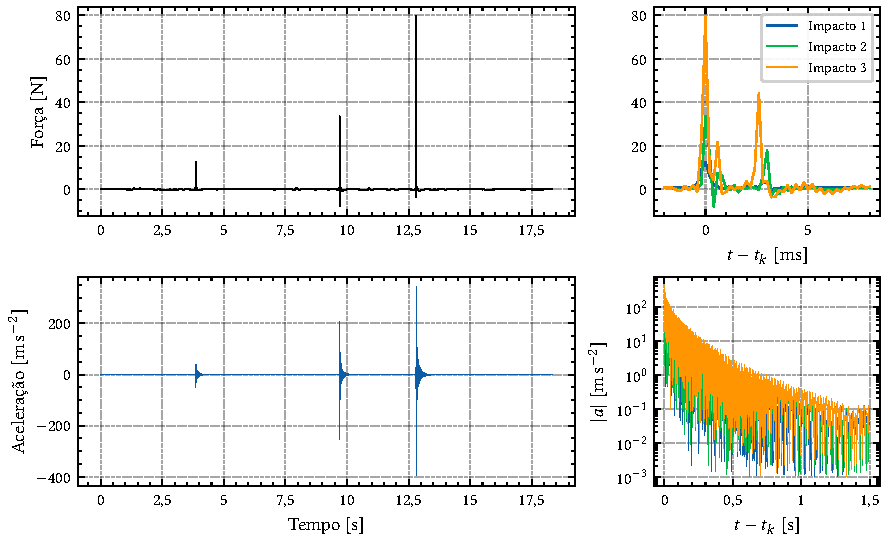
\includegraphics[width=\textwidth]{martelo_serie.pdf}
    \caption{Série temporal do ensaio com martelo. À esquerda, força e aceleração ao
        longo de todo o registro; à direita, detalhe dos pulsos de força (com o duplo
        impacto dos golpes 2 e 3) e decaimento de $|a(t)|$ após cada impacto $t_k$.}
    \label{fig:martelo_serie}
\end{figure}

Com os espectros $F_k(f)$ e $A_k(f)$ de força e aceleração de cada impacto $k$, os
autoespectros e o espectro cruzado são somados sobre os impactos,
\begin{equation}
    G_{ff} = \sum_k |F_k|^2, \qquad G_{aa} = \sum_k |A_k|^2, \qquad
    G_{fa} = \sum_k F_k^{*} A_k,
\end{equation}
e as FRFs e a coerência são \cite{ewins2000}
\begin{equation}
    H_1 = \frac{G_{fa}}{G_{ff}}, \qquad
    H_2 = \frac{G_{aa}}{G_{fa}^{*}}, \qquad
    \gamma^2 = \frac{|G_{fa}|^2}{G_{ff}\,G_{aa}} = \frac{H_1}{H_2}.
    \label{eq:estimadores}
\end{equation}
$H_1$ minimiza o efeito de ruído na resposta e $H_2$, o de ruído na força; a
coerência $\gamma^2 \le 1$ indica quanto da resposta é explicada linearmente pela
força medida. O Código~\ref{lst:frf_serie} implementa esse cálculo.

\trecho[label={lst:frf_serie}]{dados.py}{frf_serie}{[FRF do martelo a partir da série temporal]FRF do martelo a partir da série
    temporal (\texttt{dados.py}).}

Um último ajuste vale para os dois ensaios. Abaixo da primeira ressonância a viga
responde quase estaticamente: $w$ fica em fase com a força e $\ddot w = -\Omega^2 w$,
logo a acelerância deve ter fase $\pi$. Nos dois arquivos a fase medida nessa faixa é
próxima de zero, o que indica que o sentido positivo da força é oposto ao do
acelerômetro (o martelo e a célula de carga medem compressão). As FRFs medidas foram,
portanto, multiplicadas por $-1$ (constante \texttt{SINAL} em \texttt{dados.py}). Essa
correção é feita uma única vez e não usa o modelo; a concordância de sinal dos picos
com as formas modais, vista na Seção~\ref{sec:molas_res}, serve depois como
verificação independente.

%=====================================================================
\subsection{Ensaio com \emph{shaker}}
\label{sec:met_shaker}

No segundo ensaio a ponta livre foi ligada ao \emph{shaker} por uma haste
(\emph{stinger}) e uma cabeça de impedância, que mede a força transmitida e a aceleração
no mesmo ponto. O controlador Dactron fez uma varredura senoidal de \SIrange{5}{2000}{\hertz}
e exportou a transmissibilidade aceleração/força e a coerência em 512 frequências com
passo logarítmico de \SI{1.18}{\percent}. Trata-se, portanto, de uma acelerância
pontual em $x = L$, comparável a \eqref{eq:acelerancia} com $x_i = x_e = L$; a unidade
(\si{\meter\per\second\squared\per\newton}) foi confirmada pelo nível em baixa
frequência, da mesma ordem do previsto pelos modelos (Seção~\ref{sec:molas_res}); se
a razão estivesse em \si{g\per\newton}, apareceria um fator de \num{9.81}. O passo de \SI{1.18}{\percent} é da mesma ordem da banda
de meia potência dos modos pouco amortecidos ($2\zeta_r \approx
\SIrange{0.4}{1.2}{\percent}$), o que limita a precisão dos fatores de amortecimento
obtidos com esse ensaio.

%=====================================================================
\subsection{Identificação de frequências naturais e amortecimento}
\label{sec:met_identificacao}

Os picos de $|H|$ foram localizados pela proeminência em escala logarítmica: só são
aceitos picos que se destacam pelo menos meia década ($\approx 3\times$) dos vales
vizinhos, o que descarta oscilações de ruído. A frequência natural é a do máximo, e o
amortecimento vem do método da meia potência \cite{ewins2000}: sendo $f_1 < f_r < f_2$
as frequências em que $|H| = |H|_{\max}/\sqrt{2}$,
\begin{equation}
    \zeta_r = \frac{f_2 - f_1}{2 f_r}.
    \label{eq:meia_potencia}
\end{equation}
Como os pontos medidos raramente caem exatamente em $|H|_{\max}/\sqrt{2}$, cada
cruzamento é interpolado entre os dois pontos vizinhos, em $\log f$
(Código~\ref{lst:meia_potencia}). A rotina também conta quantos pontos medidos caem
dentro da banda $[f_1, f_2]$; com um ou dois pontos, a estimativa de $\zeta_r$ depende
mais da posição da grade de frequências do que do sistema.

\trecho[label={lst:meia_potencia}]{identificacao.py}{meia_potencia}{[Picos e método da meia potência]Picos e
    amortecimento pelo método da meia potência (\texttt{identificacao.py}).}

Os picos identificados são associados aos modos de flexão do modelo pela frequência
mais próxima, com tolerância de \SI{20}{\percent}; picos sem correspondente são
listados à parte.

%=====================================================================
\subsection{Solução numérica do modelo}
\label{sec:met_modelo}

As equações características \eqref{eq:car_engaste} e \eqref{eq:car_molas} crescem
como $\cosh\lambda$, que passa de $10^{8}$ para $\lambda > 20$. Para trabalhar com uma
função de ordem 1, ambas foram divididas por $\cosh\lambda$ e, no caso das molas,
também por $1 + \alpha_L\alpha_R > 0$; nenhuma das divisões altera as raízes. As
raízes são isoladas por uma varredura de sinal em $\lambda \in (0, 9\pi]$, com passo
$10^{-3}$, e refinadas pelo método de Brent, que combina bisseção com interpolação e
mantém a garantia de convergência da bisseção (Código~\ref{lst:eq_caracteristica}).
A implementação reproduz as raízes clássicas da viga engastada-livre
($\num{1.8751}$; $\num{4.6941}$; $\num{7.8548}$; \dots) e os valores do
Código~\ref{lst:normalizacao} ($\mu = \num{0.3}$, $\kappa_R = 20$,
$\kappa_L = 500$: $\lambda_r = \num{1.4730}$; $\num{3.9111}$; $\num{6.3592}$).

\trecho[label={lst:eq_caracteristica}]{modelo.py}{eq_caracteristica}{[Equações características e raízes]Equações
    características e cálculo das raízes (\texttt{modelo.py}).}

As formas modais seguem \eqref{eq:F_engaste} e \eqref{eq:F_molas}, normalizadas por
\eqref{eq:Wr_norm} com a integral calculada pela regra do trapézio em 4001 pontos.
Para os casos testados, a matriz de massa
$\int_0^L \rho A\,W_rW_s\,\mathrm{d}x + m\,W_r(L)W_s(L)$ difere da identidade em menos
de $10^{-6}$. A acelerância \eqref{eq:acelerancia} é truncada em 8 modos, o que vai
até \SI{3.9}{\kilo\hertz} no modelo com molas e \SI{4.9}{\kilo\hertz} no engastado,
acima da faixa medida (Códigos~\ref{lst:modos} e~\ref{lst:frf_num}). Os fatores
$\zeta_r$ são os identificados em cada ensaio. Na comparação com o martelo, os modos 7
e 8, sem $\zeta_r$ medido, recebem a média dos modos 3 a 6 (\SI{0.30}{\percent}); na
comparação com o \emph{shaker}, os modos 5 a 8 recebem os mesmos valores usados para o
martelo.

\trecho[label={lst:modos}]{modelo.py}{modos}{[Formas modais normalizadas]Formas modais normalizadas pela massa
    (\texttt{modelo.py}).}

\trecho[label={lst:frf_num}]{modelo.py}{frf}{[Acelerância analítica]Acelerância analítica truncada
    (\texttt{modelo.py}).}

%=====================================================================
\subsection{Ajuste da base elástica}
\label{sec:met_ajuste}

O modelo com molas tem dois parâmetros livres, $\kappa_R$ e $\kappa_L$. Eles foram
determinados impondo que as duas primeiras frequências naturais do modelo sejam iguais
às medidas no ensaio com martelo,
\begin{equation}
    f_1(\kappa_R, \kappa_L) = f_{1,\mathrm{med}}, \qquad
    f_2(\kappa_R, \kappa_L) = f_{2,\mathrm{med}},
    \label{eq:ajuste}
\end{equation}
e os modos 3 a 6 ficaram reservados para validação. O ensaio com martelo foi usado
como referência porque nele a ponta está livre, como no modelo com $m = 0$, e porque
sua FRF recalculada tem a melhor resolução e o maior número de modos. Para efeito de
comparação, o ajuste também foi repetido com os dois primeiros picos do
\emph{shaker}.

As rigidezes variam por ordens de grandeza entre uma base muito flexível e o engaste,
então as incógnitas do Código~\ref{lst:ajuste} são $\log_{10}\kappa_R$ e
$\log_{10}\kappa_L$, o que também as mantém positivas. Os resíduos são os erros
relativos $f_r/f_{r,\mathrm{med}} - 1$, e o sistema \eqref{eq:ajuste} é resolvido por
mínimos quadrados (região de confiança), com tolerâncias de $10^{-12}$; na solução os
resíduos são nulos. Para avaliar a robustez do resultado, o ajuste foi refeito com
$f_1$ ou $f_2$ alteradas em $\pm\SI{1}{\percent}$, variação comparável às diferenças
entre os dois ensaios e ao efeito de massas pequenas como a do acelerômetro.

\trecho[label={lst:ajuste}]{ajuste_molas.py}{ajuste}{[Ajuste da base elástica]Ajuste de $\kappa_R$ e $\kappa_L$
    às duas primeiras frequências e validação (\texttt{ajuste\_molas.py}).}

\FloatBarrier

\section{Resultados e discussão}
\label{sec:resultados}

%=====================================================================
\subsection{FRFs experimentais}
\label{sec:frf_exp}

\subsubsection{Ensaio com martelo}

A Figura~\ref{fig:frf_martelo} mostra a acelerância do ensaio com martelo, com módulo,
fase e coerência. Aparecem seis picos de flexão na faixa medida, em \num{25.2}; \num{164.1};
\num{459.0}; \num{893.2}; \num{1462.3} e \SI{2157.5}{\hertz}. Os
estimadores $H_1$ e $H_2$ praticamente coincidem onde a coerência é próxima de 1 e
só se separam nas antirressonâncias e abaixo de \SI{20}{\hertz}, onde a resposta é
pequena e o ruído pesa mais; nessas faixas a coerência cai, como esperado. Os picos
têm coerência acima de \num{0.96}, com duas exceções: o modo 3 (\num{0.84}), que é
fraco porque o ponto de impacto fica muito perto de um nó desse modo
(Figura~\ref{fig:modos}), e o modo 5 (\num{0.60}), vizinho de uma antirressonância
em torno de \SI{1.5}{\kilo\hertz}.

\begin{figure}[htbp]
    \centering
    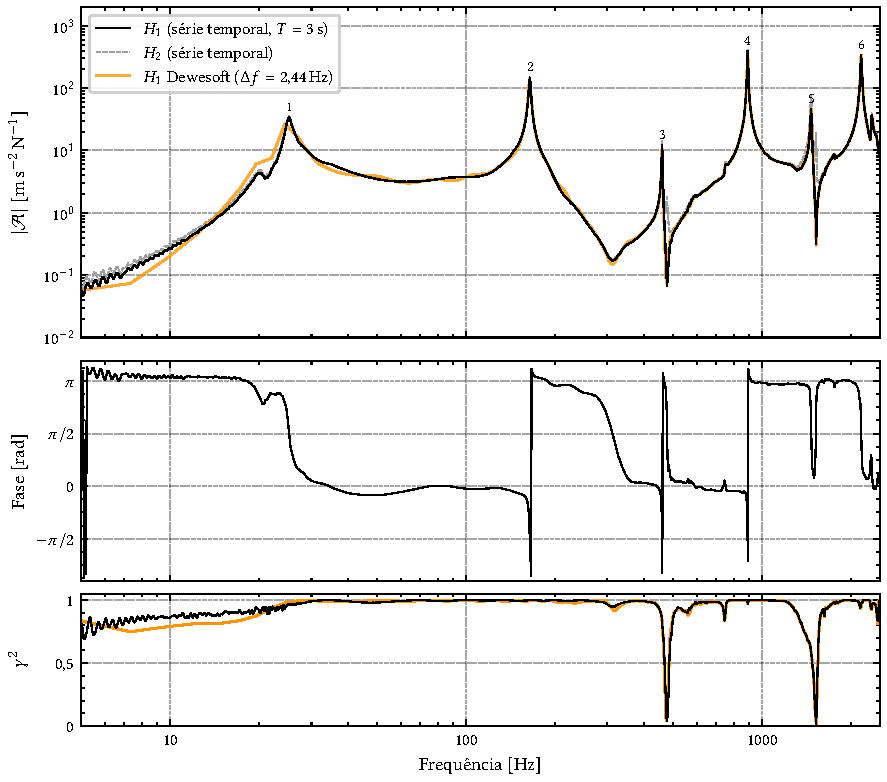
\includegraphics[width=\textwidth]{frf_martelo.pdf}
    \caption{Acelerância $\ddot w(x_e)/f(x_i)$ do ensaio com martelo ($x_i =
            \SI{0.200}{\meter}$, $x_e = \SI{0.356}{\meter}$): módulo, fase de $H_1$ e
        coerência. Em preto e cinza, $H_1$ e $H_2$ recalculados da série temporal; em
        laranja, $H_1$ exportado pelo Dewesoft. Os números indicam os modos de flexão.}
    \label{fig:frf_martelo}
\end{figure}

A curva exportada pelo Dewesoft concorda com a recalculada em quase toda a faixa,
mas não no primeiro modo, em que o pico fica mais baixo e mais largo. A
Tabela~\ref{tab:resolucao} quantifica a diferença. Com $\Delta f = \SI{2.44}{\hertz}$
e registros de \SI{0.41}{\second}, a banda de meia potência do modo 1 contém um único
ponto, e a meia potência dá $\zeta_1 = \SI{6.1}{\percent}$; com a FRF recalculada,
há 32 pontos na banda e $\zeta_1 = \SI{2.40}{\percent}$. A partir do modo 2 as duas
estimativas de frequência diferem menos de \SI{1}{\hertz}, e as de amortecimento
convergem à medida que a banda passa a conter mais pontos. As frequências e
amortecimentos do martelo usados daqui em diante são os da FRF recalculada.

\begin{table}[htbp]
    \centering
    \caption{Ensaio com martelo: parâmetros modais obtidos da FRF exportada pelo
        Dewesoft e da FRF recalculada a partir da série temporal. $n$ é o número de
        pontos dentro da banda de meia potência.}
    \label{tab:resolucao}
    \begin{tabular}{c rrr rrrr}
        \toprule
             & \multicolumn{3}{c}{Dewesoft ($\Delta f = \SI{2.44}{\hertz}$)}
             & \multicolumn{4}{c}{Série temporal ($T = \SI{3}{\second}$)}                                                    \\
        \cmidrule(lr){2-4}\cmidrule(lr){5-8}
        Modo & $f_r$ [\si{\hertz}] & $\zeta_r$ [\si{\percent}] & $n$
             & $f_r$ [\si{\hertz}] & $\zeta_r$ [\si{\percent}] & $n$ & $\gamma^2$                                          \\
        \midrule
        \linhas{martelo_resolucao}
        \bottomrule
    \end{tabular}
\end{table}

A fase confirma a identificação dos modos. Numa FRF de transferência, cada modo
contribui com $W_r(x_e)W_r(x_i)/(\omega_r^2 - \Omega^2 + 2\iu\zeta_r\omega_r\Omega)$,
e a fase da acelerância na ressonância é $+\pi/2$ se a constante modal
$W_r(x_e)W_r(x_i)$ for positiva e $-\pi/2$ se for negativa. Os modos 1, 5 e 6 passam
por $+\pi/2$ e os modos 2, 3 e 4 por $-\pi/2$. Essa sequência é comparada com os
modelos na Seção~\ref{sec:molas_res}. Há ainda um pequeno pico em
\SI{20.3}{\hertz}, abaixo do primeiro modo, que não corresponde a nenhum modo de
flexão da viga; ele reaparece no ensaio com \emph{shaker} e é discutido adiante.

\subsubsection{Ensaio com \emph{shaker}}

A Figura~\ref{fig:frf_shaker} mostra a acelerância pontual medida na ponta. Como
força e aceleração são medidas no mesmo ponto, todas as constantes modais
$W_r(L)^2$ são positivas: ressonâncias e antirressonâncias se alternam e a fase fica
entre 0 e $\pi$, passando por $\pi/2$ em cada ressonância \cite{ewins2000}. Os dados
seguem esse padrão. Há quatro picos associados a modos de flexão (\num{24.1}; \num{160.8};
\num{495.5} e \SI{966.8}{\hertz}) e um quinto, em \SI{387.4}{\hertz} (marcado com ``?''), que forma
um par quase coincidente com uma antirressonância em \SI{383}{\hertz} e não tem
correspondente no ensaio com martelo nem nos modelos. Um par polo--zero tão próximo
indica um modo que quase não participa da resposta na ponta; é provável que venha do
conjunto \emph{shaker}--haste ou de um modo que não é de flexão vertical (torção ou
flexão lateral) excitado por algum desalinhamento. Esse pico foi excluído da comparação
com os modelos.

\begin{figure}[htbp]
    \centering
    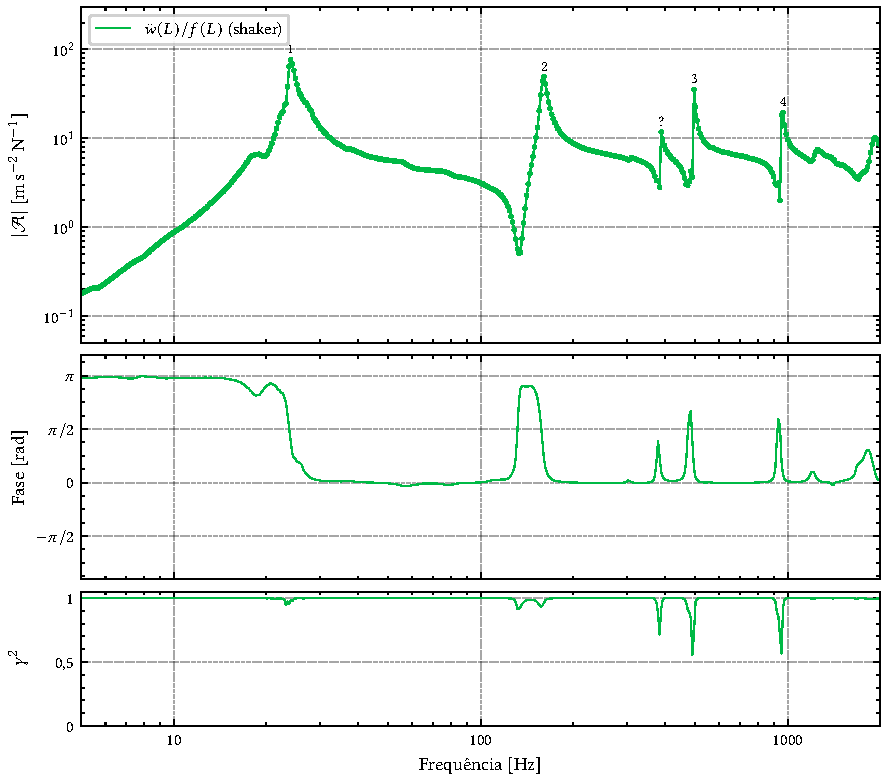
\includegraphics[width=\textwidth]{frf_shaker.pdf}
    \caption{Acelerância pontual $\ddot w(L)/f(L)$ do ensaio com \emph{shaker}: módulo,
        fase e coerência. Os pontos são as 512 frequências da varredura.}
    \label{fig:frf_shaker}
\end{figure}

Nos dois ensaios aparece também uma pequena ressonância isolada abaixo do primeiro
modo, em \SI{20.3}{\hertz} no martelo e em torno de \SI{19}{\hertz} no
\emph{shaker}, com uma perturbação localizada na fase. Ela não é prevista por nenhum
modelo da viga, e sua presença nas duas montagens, com excitações diferentes, sugere
um modo da estrutura de suporte. Isso é um indício direto de que a base não é
perfeitamente rígida.

%=====================================================================
\subsection{Frequências naturais e amortecimento: martelo \texorpdfstring{$\times$}{x} \emph{shaker}}
\label{sec:comparacao_ensaios}

A Tabela~\ref{tab:martelo_shaker} compara os parâmetros modais dos dois ensaios.

\begin{table}[htbp]
    \centering
    \caption{Frequências naturais e fatores de amortecimento identificados nos dois
        ensaios. $n$ é o número de pontos medidos na banda de meia potência do
        \emph{shaker}, e $\Delta f$, a diferença relativa entre as frequências do
        \emph{shaker} e do martelo.}
    \label{tab:martelo_shaker}
    \begin{tabular}{c rr rrrr r}
        \toprule
             & \multicolumn{2}{c}{Martelo} & \multicolumn{4}{c}{\emph{Shaker}} &                                                   \\
        \cmidrule(lr){2-3}\cmidrule(lr){4-7}
        Modo & $f_r$ [\si{\hertz}]         & $\zeta_r$ [\si{\percent}]         & $f_r$ [\si{\hertz}] & $\zeta_r$ [\si{\percent}]
             & $n$                         & $\gamma^2$                        & $\Delta f$ [\si{\percent}]                         \\
        \midrule
        \linhas{martelo_shaker}
        \bottomrule
    \end{tabular}
\end{table}

\paragraph{Frequências.} Os dois primeiros modos do \emph{shaker} ficam
\SI{4.6}{\percent} e \SI{2.0}{\percent} abaixo dos do martelo, enquanto os modos 3 e 4
ficam cerca de \SI{8}{\percent} acima. As duas montagens não são, portanto, o mesmo
sistema. No ensaio com \emph{shaker}, a cabeça de impedância e sua fixação acrescentam
massa à ponta, o que reduz as frequências. Usando o modelo com base elástica ajustado
na Seção~\ref{sec:molas_res}, uma massa de \SI{17}{\gram} na ponta reproduziria a
queda do modo 1, mas também reduziria os modos 2, 3 e 4 em \SI{4.3}{\percent},
\SI{3.9}{\percent} e \SI{3.3}{\percent}. Como os modos 3 e 4 medidos sobem, a ligação
deve também restringir a ponta: a haste e a cabeça de impedância transmitem momento e
dificultam a rotação da extremidade, o que enrijece sobretudo os modos mais altos,
cuja forma tem grande rotação na ponta. A célula de carga mede só a força axial da
haste; o momento transmitido não entra na FRF medida, de modo que esse efeito aparece
como uma mudança no próprio sistema ensaiado. Por isso o ensaio com martelo, com a
ponta realmente livre, é a referência para o ajuste do modelo.

\paragraph{Amortecimento.} No martelo, o primeiro modo tem
$\zeta_1 = \SI{2.40}{\percent}$, bem mais que os demais
(\SIrange{0.20}{0.61}{\percent}). O \emph{shaker} confirma esse valor
($\zeta_1 = \SI{2.21}{\percent}$, com 4 pontos na banda), mas dá amortecimentos 3 a 6
vezes maiores nos modos 2 a 4. Esses valores do \emph{shaker} não são confiáveis: com
passo de \SI{1.18}{\percent}, a banda de meia potência desses modos contém de 1 a 3
pontos, o ponto mais alto medido fica, em geral, abaixo do pico real, e a banda
estimada resulta mais larga. Além disso, na ressonância a impedância da viga na ponta
é mínima e o \emph{shaker} consegue impor pouca força, o que reduz a relação
sinal--ruído justamente no pico (a coerência do modo 3, \num{0.73}, é a mais baixa).
Os fatores do martelo, obtidos com dezenas a centenas de pontos por banda, são
adotados como representativos da viga. O amortecimento maior do modo 1 é compatível
com dissipação no engaste parafusado: no modelo ajustado na
Seção~\ref{sec:molas_res}, é no modo 1 que a mola torcional da base armazena a maior
parcela da energia de deformação (\SI{35}{\percent}, contra no máximo
\SI{17}{\percent} nos demais modos). Também pode contribuir a troca de energia com o
modo do suporte em torno de \SI{20}{\hertz}, vizinho de $f_1$. Os dados não permitem
separar essas contribuições.

%=====================================================================
\subsection{Efeito da massa na ponta}
\label{sec:massa}

Os ensaios foram feitos sem a massa concentrada de \SI{0.445}{\kilo\gram}. Para
avaliar quanto as frequências teriam mudado com ela, os dois modelos foram resolvidos
com $\mu = \num{0.705}$, mantendo as mesmas condições na base: o engaste ideal e a base
elástica ajustada na Seção~\ref{sec:molas_res}. A Tabela~\ref{tab:massa} e a
Figura~\ref{fig:massa} mostram o resultado.

\begin{table}[htbp]
    \centering
    \caption{Frequências naturais [\si{\hertz}] sem massa ($\mu = 0$) e com a massa de
        \SI{0.445}{\kilo\gram} na ponta ($\mu = \num{0.705}$), para as duas condições de
        base, e variação relativa causada pela massa.}
    \label{tab:massa}
    \begin{tabular}{c r rrr rrr}
        \toprule
             &          & \multicolumn{3}{c}{Base engastada} & \multicolumn{3}{c}{Base elástica ajustada}                                                                        \\
        \cmidrule(lr){3-5}\cmidrule(lr){6-8}
        Modo & Medido   & $\mu = 0$                          & $\mu = \num{0.705}$                        & Var. [\si{\percent}] & $\mu = 0$ & $\mu = \num{0.705}$ & Var. [\si{\percent}] \\
        \midrule
        \linhas{massa_ponta}
        \bottomrule
    \end{tabular}
\end{table}

\begin{figure}[htbp]
    \centering
    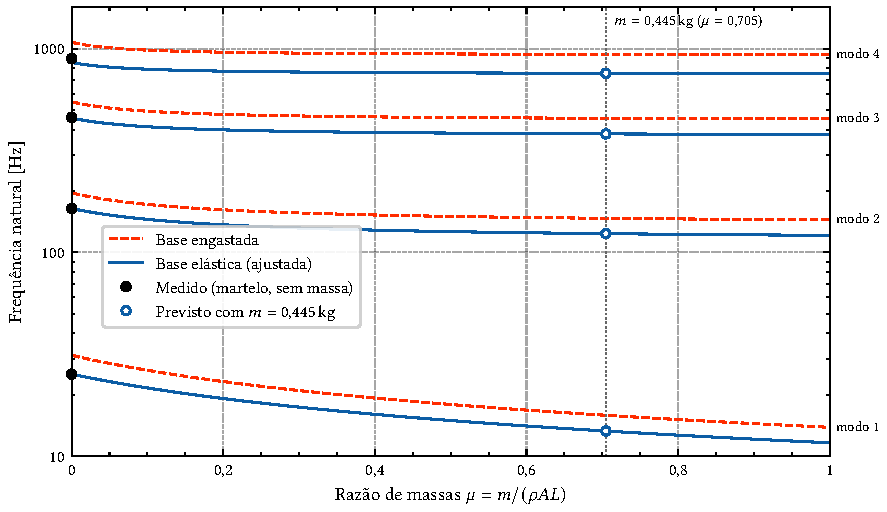
\includegraphics[width=\textwidth]{massa_ponta.pdf}
    \caption{Frequências naturais dos quatro primeiros modos em função da razão de
        massas $\mu$, para a base engastada e para a base elástica ajustada. Os pontos
        cheios são as frequências medidas (sem massa); os vazados, as previstas com a
        massa de \SI{0.445}{\kilo\gram}.}
    \label{fig:massa}
\end{figure}

Com a massa, o primeiro modo cairia quase pela metade, para \SI{15.8}{\hertz} com
engaste ideal e \SI{13.3}{\hertz} com a base elástica, e o segundo cairia
\SI{25}{\percent}, para \num{146.8} e \SI{123.4}{\hertz}. O efeito diminui nos modos
mais altos (\SIrange{8}{17}{\percent} nos modos 3 a 6). A massa fica onde todos os
modos têm amplitude máxima, mas seu efeito depende de quanto ela pesa em relação à
massa que participa de cada modo. No modo 1 a viga inteira se move em fase, e a massa
modal efetiva na ponta é cerca de um quarto da massa da viga, bem menor que
\SI{0.445}{\kilo\gram}. Nos modos altos, a massa grande praticamente impede a
translação da ponta, e as curvas da Figura~\ref{fig:massa} tendem aos modos de uma
viga engastada-apoiada: com $\mu \to \infty$, o modo $r$ tende ao modo $r - 1$ dessa
viga ($\lambda = \num{3.927}$; $\num{7.069}$; $\num{10.21}$; \dots), o que explica o
achatamento das curvas.

A comparação também confirma que o ensaio foi feito sem a massa. Qualquer
flexibilidade na base só reduz as frequências, de modo que o engaste ideal dá o maior
valor possível para cada modo. Com a massa, esse limite seria \SI{15.8}{\hertz} para
o modo 1 e \SI{146.8}{\hertz} para o modo 2, e o medido é \num{25.2} e
\SI{164.1}{\hertz}, acima dos dois limites. Os modos 3 e 4 do engaste com massa
(\num{454.7} e \SI{936.7}{\hertz}) ficam próximos dos medidos (\num{459.0} e
\SI{893.2}{\hertz}), mas isso é coincidência: são justamente os modos menos sensíveis
à massa, e não servem para discriminar as hipóteses. Os modos 1 e 2, os mais sensíveis,
são incompatíveis com ela.

%=====================================================================
\subsection{Condição de contorno: engaste ideal \texorpdfstring{$\times$}{x} base elástica}
\label{sec:molas_res}

\subsubsection{Engaste ideal}

O modelo engastado superestima todas as frequências medidas, de \SI{19}{\percent} a
\SI{24}{\percent} (Tabela~\ref{tab:validacao}). A FRF analítica correspondente
(Figura~\ref{fig:frf_martelo_modelos}) tem a forma certa, com a mesma sequência de
picos e antirressonâncias, mas deslocada para a direita, e fica abaixo da medida em
baixa frequência: a viga real é mais flexível que uma viga perfeitamente engastada.

\subsubsection{Ajuste da base elástica}

Resolvendo \eqref{eq:ajuste} com $f_{1,\mathrm{med}} = \SI{25.22}{\hertz}$ e
$f_{2,\mathrm{med}} = \SI{164.07}{\hertz}$, obtém-se
\begin{equation}
    \kappa_R = \vkapR, \qquad \kappa_L = \vkapL,
    \label{eq:molas_ajustadas}
\end{equation}
ou, em unidades físicas,
$k_R = \kappa_R EI/L = \SI{2.79e3}{\newton\meter\per\radian}$ e
$k_L = \kappa_L EI/L^3 = \SI{2.84e6}{\newton\per\meter}$.
A Figura~\ref{fig:ajuste} mostra o problema de ajuste no plano
$(\log_{10}\kappa_R, \log_{10}\kappa_L)$. As curvas $f_1 = f_{1,\mathrm{med}}$ e
$f_2 = f_{2,\mathrm{med}}$ se cruzam em um único ponto da região explorada. Para
$\kappa_L$ grande as duas ficam quase verticais, isto é, passam a depender só de
$\kappa_R$, e elas se cruzam com um ângulo pequeno. Na solução, uma década em
$\kappa_R$ muda $f_1$ em \SI{40}{\percent} e $f_2$ em \SI{19}{\percent}, enquanto uma
década em $\kappa_L$ muda $f_1$ em apenas \SI{0.4}{\percent} e $f_2$ em
\SI{5.4}{\percent}. Por isso $\kappa_R$ fica bem determinado, mas $\kappa_L$ não: uma
variação de \SI{1}{\percent} em $f_2$ leva $\kappa_L$ de cerca de \num{1000} a
\num{2600} (Tabela~\ref{tab:sensibilidade}). O ajuste com os dois primeiros picos do
\emph{shaker} dá $\kappa_R = \vkapRs$ e $\kappa_L = \vkapLs$: o mesmo $\kappa_L$
dentro dessa incerteza e um $\kappa_R$ menor, coerente com o $f_1$ do \emph{shaker}
rebaixado pela massa da cabeça de impedância.

\begin{figure}[htbp]
    \centering
    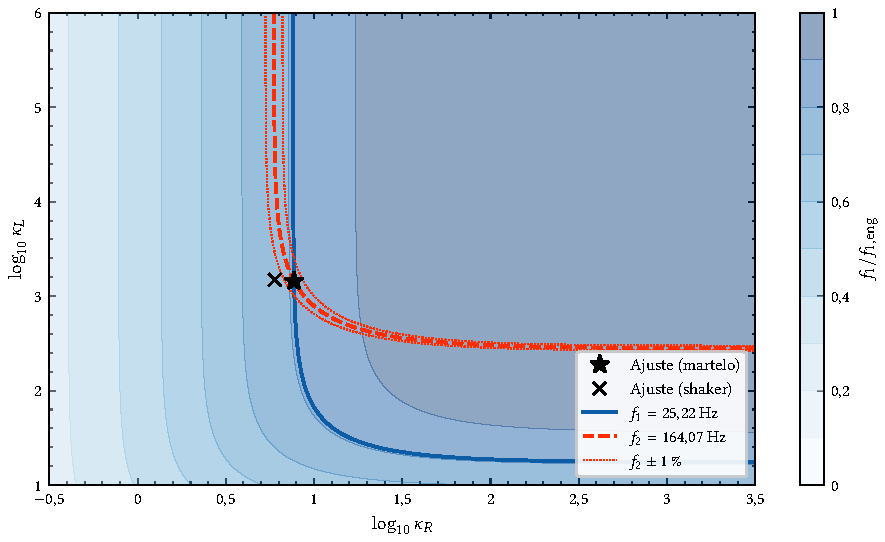
\includegraphics[width=\textwidth]{ajuste_molas.pdf}
    \caption{Ajuste da base elástica. Curvas de $f_1$ e $f_2$ iguais às medidas no
        martelo, no plano das rigidezes adimensionais; as linhas pontilhadas
        correspondem a $f_2 \pm \SI{1}{\percent}$. O fundo mostra $f_1$ relativo ao
        engaste ideal.}
    \label{fig:ajuste}
\end{figure}

O valor de $\kappa_R$ diz que a fixação tem rigidez à rotação de apenas
$\num{7.7}\,EI/L$. Estaticamente, a flexibilidade na ponta de uma viga com essas
molas é $\frac{L^3}{3EI}\left(1 + 3/\kappa_R + 3/\kappa_L\right)$, ou
\SI{39}{\percent} maior que a do engaste, e quase todo o acréscimo
($3/\kappa_R = \num{0.39}$) vem da rotação da base. A mola transversal é
estaticamente desprezível ($3/\kappa_L = \num{0.002}$), mas não dinamicamente: a
rigidez adimensional que conta em cada modo é $\alpha_L = \kappa_L/\lambda^3$
\eqref{eq:alphas}, que cai de cerca de \num{300} no modo 1 para \num{1.5} no modo 4.
Nos modos altos a base passa a transladar de forma apreciável
(Figura~\ref{fig:modos}). As duas molas são necessárias: uma mola torcional sozinha
($\kappa_L \to \infty$) ajustada a $f_1$ exige $\kappa_R = \num{7.61}$, mas
superestima $f_2$ em \SI{2.3}{\percent} e os modos 3 a 6 em \SIrange{5.8}{14.4}{\percent}.

\subsubsection{Validação com os modos 3 a 6}

A Tabela~\ref{tab:validacao} e a Figura~\ref{fig:validacao} comparam as previsões dos
dois modelos com os modos que não entraram no ajuste.

\begin{table}[htbp]
    \centering
    \caption{Frequências naturais medidas (martelo) e previstas [\si{\hertz}], erro
        relativo $e_r = f_{r,\mathrm{mod}}/f_{r,\mathrm{med}} - 1$ e razão entre a
        frequência medida e a do engaste ideal.}
    \label{tab:validacao}
    \begin{tabular}{c r rr rr r l}
        \toprule
             &         & \multicolumn{2}{c}{Engaste} & \multicolumn{2}{c}{Base elástica} &                                                                                                  \\
        \cmidrule(lr){3-4}\cmidrule(lr){5-6}
        Modo & Medido  & $f_r$                       & $e_r$ [\si{\percent}]              & $f_r$ & $e_r$ [\si{\percent}] & $f_{\mathrm{med}}/f_{\mathrm{eng}}$ & Uso       \\
        \midrule
        \linhas{validacao}
        \bottomrule
    \end{tabular}
\end{table}

\begin{figure}[htbp]
    \centering
    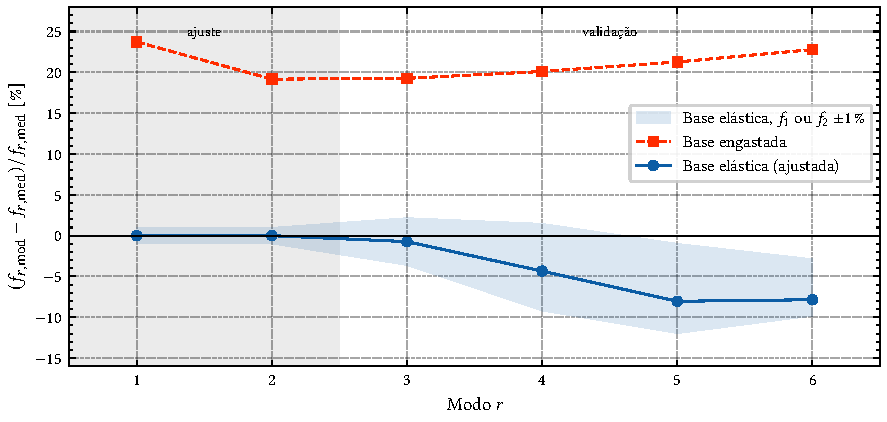
\includegraphics[width=\textwidth]{validacao.pdf}
    \caption{Erro relativo das frequências previstas pelos dois modelos. A faixa azul
        mostra a variação do erro da base elástica quando o ajuste é refeito com $f_1$
        ou $f_2$ alteradas em $\pm\SI{1}{\percent}$.}
    \label{fig:validacao}
\end{figure}

\begin{table}[htbp]
    \centering
    \caption{Sensibilidade do ajuste: rigidezes e erros de validação [\si{\percent}]
        quando $f_1$ ou $f_2$ é alterada em $\pm\SI{1}{\percent}$ antes do ajuste.}
    \label{tab:sensibilidade}
    \begin{tabular}{l rr rrrr}
        \toprule
        Perturbação & $\kappa_R$ & $\kappa_L$ & $e_3$ & $e_4$ & $e_5$ & $e_6$ \\
        \midrule
        Nenhuma     & \vkapR     & \vkapL     & \num{-0.7} & \num{-4.3} & \num{-8.0} & \num{-7.8} \\
        \linhas{sensibilidade}
        \bottomrule
    \end{tabular}
\end{table}

A base elástica reduz o erro do modo 3 de \SI{+19.3}{\percent} para
\SI{-0.7}{\percent} e o do modo 4 de \SI{+20.1}{\percent} para \SI{-4.3}{\percent}.
Nos modos 5 e 6 o erro cai de cerca de \SI{+22}{\percent} para cerca de
\SI{-8}{\percent}. Considerando a sensibilidade da Tabela~\ref{tab:sensibilidade}, os
erros dos modos 3 e 4 são compatíveis com zero para variações de \SI{1}{\percent} nas
frequências de ajuste, comparáveis, por exemplo, ao efeito da massa do acelerômetro
ou à diferença entre os dois ensaios. Já os modos 5 e 6 ficam abaixo do medido em
todos os casos (de \SI{-1}{\percent} a \SI{-12}{\percent}): o modelo ajustado é
flexível demais nos modos altos.

A Figura~\ref{fig:frf_martelo_modelos} compara as FRFs. Com a base elástica, as posições
dos três primeiros picos e o nível da FRF em baixa frequência coincidem com os
medidos, e a altura dos picos 1 e 2, calculada com os $\zeta_r$ do martelo, é da mesma
ordem da medida. O pico 3 do modelo elástico quase não aparece, porque sua constante
modal é praticamente nula (Tabela~\ref{tab:sinais}). A partir do modo 4 os picos do modelo ficam à esquerda dos medidos, como na
Tabela~\ref{tab:validacao}. No \emph{shaker} (Figura~\ref{fig:frf_shaker_modelos}), o
modelo elástico se aproxima dos dois primeiros picos, enquanto os modos 3 e 4 medidos
ficam acima até do engaste, coerente com a restrição na ponta discutida na
Seção~\ref{sec:comparacao_ensaios}. Pela mesma razão, o nível medido em baixa
frequência fica mais perto do modelo engastado: a ligação com o \emph{shaker}
enrijece a ponta. Os picos do \emph{shaker} são mais baixos que os do modelo porque a
varredura não amostra o topo dos picos estreitos.

\begin{figure}[htbp]
    \centering
    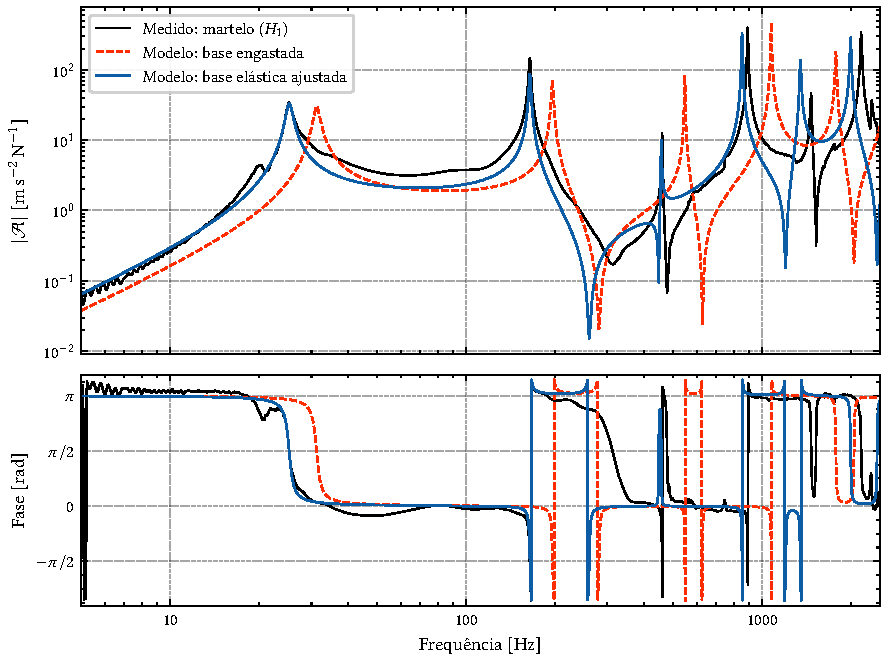
\includegraphics[width=\textwidth]{frf_martelo_modelos.pdf}
    \caption{FRF do ensaio com martelo comparada às acelerâncias analíticas
        \eqref{eq:acelerancia} com base engastada e com base elástica ajustada, ambas com
        os $\zeta_r$ identificados no martelo.}
    \label{fig:frf_martelo_modelos}
\end{figure}

\begin{figure}[htbp]
    \centering
    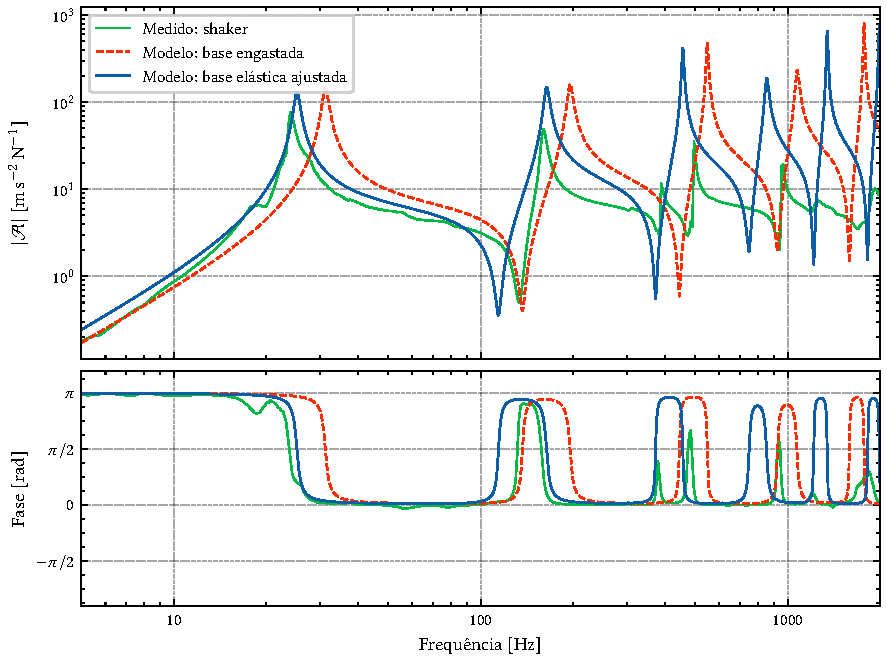
\includegraphics[width=\textwidth]{frf_shaker_modelos.pdf}
    \caption{FRF pontual do ensaio com \emph{shaker} comparada às acelerâncias
        analíticas em $x_i = x_e = L$, com os $\zeta_r$ identificados no
        \emph{shaker}.}
    \label{fig:frf_shaker_modelos}
\end{figure}

\subsubsection{Formas modais e sinais das constantes modais}

A Figura~\ref{fig:modos} mostra os quatro primeiros modos normalizados dos dois
modelos. Com a base elástica, a base gira em todos os modos e passa a transladar nos
modos 3 e 4, e os nós se deslocam em direção à base. Isso altera o sinal da constante
modal $W_r(x_e)W_r(x_i)$ em alguns modos, que pode ser comparado com a fase medida na
ressonância (Tabela~\ref{tab:sinais}). O engaste reproduz o sinal medido nos seis
modos. O modelo elástico acerta os modos 1, 2, 4 e 6, mas erra os modos 3 e 5. No modo
3, o ponto de impacto fica perto de um nó nos dois modelos (em \SI{0.217}{\meter} no
engaste e em \SI{0.196}{\meter} na base elástica), e a constante modal é a menor de
todas, o que explica o pico fraco desse modo; um pequeno deslocamento do nó basta para
trocar o sinal, de modo que esse desacordo pesa pouco. No modo
5, porém, a diferença é clara: o engaste prevê constante positiva, como a medida, e a
base elástica, negativa.

\begin{figure}[htbp]
    \centering
    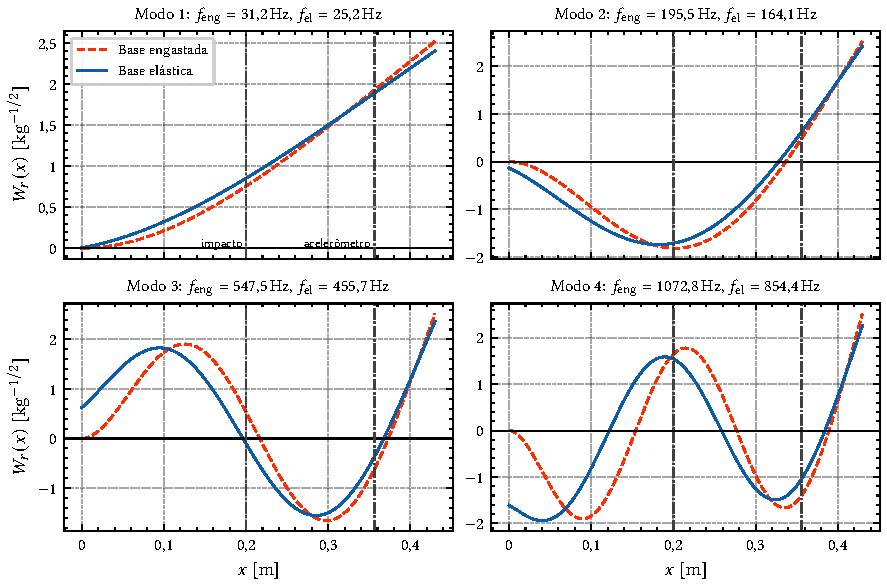
\includegraphics[width=\textwidth]{modos.pdf}
    \caption{Quatro primeiros modos normalizados pela massa, para a base engastada e
        para a base elástica ajustada, com a convenção $W_r(L) > 0$. As linhas
        traço-ponto marcam o ponto de impacto ($x = \SI{0.200}{\meter}$) e o
        acelerômetro ($x = \SI{0.356}{\meter}$).}
    \label{fig:modos}
\end{figure}

\begin{table}[htbp]
    \centering
    \caption[Fase medida nos picos e sinal das constantes modais]{Fase medida no
        pico de cada modo (martelo) e constante modal
        $W_r(x_e)W_r(x_i)$ [\si{\per\kilo\gram}] prevista pelos dois modelos. Fase
        $+\pi/2$ corresponde a constante positiva.}
    \label{tab:sinais}
    \begin{tabular}{c rc rr}
        \toprule
        Modo & Fase medida [\si{\radian}] & Sinal & Engaste & Base elástica \\
        \midrule
        \linhas{sinais}
        \bottomrule
    \end{tabular}
\end{table}

\subsubsection{Qual condição de contorno é adequada?}

Entre as duas hipóteses pedidas no roteiro, a base elástica é claramente a mais
adequada para prever frequências: com dois parâmetros ajustados aos dois primeiros
modos, ela reduz os erros de cerca de \SI{20}{\percent} para menos de
\SI{1}{\percent} no modo 3 e \SI{4.3}{\percent} no modo 4, e reproduz o nível da FRF
em baixa frequência. O engaste ideal é rígido demais em todos os modos. A rigidez à
rotação da fixação, $k_R \approx \SI{2.8e3}{\newton\meter\per\radian}$, é a parte bem
determinada do ajuste e explica a maior parte da diferença.

O modelo de molas, porém, não explica tudo. Três observações indicam que parte da
discrepância não vem só da fixação: (i) a razão $f_{\mathrm{med}}/f_{\mathrm{eng}}$ é
quase constante nos seis modos (\numrange{0.81}{0.84}, Tabela~\ref{tab:validacao}),
enquanto molas na base afetam modos diferentes de forma diferente; (ii) o modelo
ajustado fica flexível demais nos modos 5 e 6; (iii) os sinais das constantes modais
seguem as formas do engaste, não as da base elástica, no modo 5. Um modelo engastado
com todas as frequências multiplicadas por um único fator de \num{0.83}, equivalente a
reduzir $EI/\rho A$ em \SI{32}{\percent} ou a um comprimento efetivo de
\SI{0.473}{\meter}, reproduziria as seis frequências com erro de no máximo
\SI{2.2}{\percent}. Isso sugere que os parâmetros nominais da viga também merecem
revisão; a própria massa $m_b$ do roteiro é inconsistente com $\rho A L$
(Seção~\ref{sec:parametros}). Separar o efeito da fixação do efeito de $EI/\rho A$
exigiria medir a espessura e a massa da viga e obter a resposta em mais pontos, de
modo a identificar as formas modais, inclusive a rotação e a translação na base.

\FloatBarrier

\section{Conclusão}
\label{sec:conclusao}

As frequências naturais e os fatores de amortecimento da viga foram identificados nos
ensaios com martelo e com \emph{shaker} e comparados com o modelo de Euler--Bernoulli
com duas condições de contorno na base. As principais conclusões são:

\begin{itemize}
    \item O ensaio com martelo identificou seis modos de flexão, em \num{25.2};
          \num{164.1}; \num{459.0}; \num{893.2}; \num{1462.3} e \SI{2157.5}{\hertz}.
          Recalcular a FRF a partir da série temporal, com registros de \SI{3}{\second}
          que contêm toda a resposta, foi essencial para o primeiro modo: a FRF exportada
          pelo Dewesoft, com $\Delta f = \SI{2.44}{\hertz}$, leva a $\zeta_1 =
          \SI{6.1}{\percent}$, contra $\SI{2.40}{\percent}$ com a FRF recalculada. Os
          demais modos têm $\zeta_r$ entre \SI{0.20}{\percent} e \SI{0.61}{\percent}.

    \item No ensaio com \emph{shaker}, os modos 1 e 2 ficam \SI{4.6}{\percent} e
          \SI{2.0}{\percent} abaixo dos do martelo e os modos 3 e 4, cerca de
          \SI{8}{\percent} acima. A ligação com o excitador acrescenta massa à ponta e
          restringe sua rotação, de modo que os dois ensaios não medem exatamente o
          mesmo sistema. Os amortecimentos do \emph{shaker} acima do primeiro modo são
          superestimados pela resolução da varredura, que deixa de 1 a 3 pontos em cada
          banda de meia potência.

    \item Os ensaios foram feitos sem a massa de \SI{0.445}{\kilo\gram} na ponta, e os
          dados confirmam isso. Com a massa, o primeiro modo cairia para no máximo
          \SI{15.8}{\hertz} (engaste ideal) e o segundo para no máximo
          \SI{146.8}{\hertz}, abaixo dos valores medidos. Com a base elástica ajustada, as
          frequências com a massa seriam \num{13.3}; \num{123.4}; \num{381.2} e
          \SI{756.3}{\hertz} nos quatro primeiros modos, reduções de
          \SIrange{47}{12}{\percent} em relação ao caso sem massa.

    \item O engaste ideal superestima todas as frequências em \SIrange{19}{24}{\percent}.
          A base elástica com $\kappa_R$ e $\kappa_L$ ajustadas aos dois primeiros picos
          ($k_R = \SI{2.8e3}{\newton\meter\per\radian}$,
          $k_L = \SI{2.8e6}{\newton\per\meter}$) prevê o modo 3 com erro de
          \SI{-0.7}{\percent} e o modo 4 com \SI{-4.3}{\percent}, e reproduz o nível da
          FRF em baixa frequência. Entre as duas hipóteses, é a condição de contorno
          adequada. A rigidez à rotação é bem determinada pelo ajuste; a rigidez
          transversal, não, e varia de \num{1000} a \num{2600} (em $\kappa_L$) com
          \SI{1}{\percent} de variação em $f_2$.

    \item O modelo ajustado subestima os modos 5 e 6 em cerca de \SI{8}{\percent}, e o
          sinal da constante modal do modo 5 só concorda com as formas do engaste. Como a
          razão entre as frequências medidas e as do engaste é quase constante
          (\numrange{0.81}{0.84}), parte da diferença deve vir dos parâmetros nominais
          da viga, e não só da fixação. Medir a espessura e a massa da viga e obter a
          resposta em mais pontos, incluindo a base, permitiria separar os dois efeitos.
\end{itemize}


% 4. Print the bibliography
\clearpage
\begingroup
\small
\setlength{\bibitemsep}{0.25\baselineskip}
\printbibliography[heading=bibintoc]
\endgroup

% 5. Apêndice: código completo
\clearpage
\appendix
\section{Código completo}
\label{ap:codigo}

Este apêndice traz o código numérico completo usado na análise. Os scripts simbólicos
da Seção~\ref{sec:intro} já aparecem por inteiro nos
Códigos~\ref{lst:solucao_geral} a~\ref{lst:frf} e não são repetidos.

Os arquivos ficam na pasta \texttt{codigo/} e leem os dados de \texttt{dados/}. Para
reproduzir as figuras e tabelas, basta executar, dentro de \texttt{codigo/},
\begin{center}
    \texttt{python gera\_resultados.py}
\end{center}
com Python 3.11 ou mais recente e os pacotes listados em \texttt{requirements.txt}
(NumPy, SciPy, Matplotlib, SciencePlots e SymPy). O estilo SciencePlots usa o
\LaTeX{} do sistema para escrever os textos das figuras. Os comentários
\texttt{\# <{}<nome>{}>} marcam os trechos reproduzidos ao longo do texto.

\lstinputlisting[caption={\texttt{parametros.py}: parâmetros da viga e conversão
            $\lambda_r \leftrightarrow f_r$.}, label={lst:ap_parametros}]{codigo/parametros.py}

\lstinputlisting[caption={\texttt{dados.py}: leitura dos arquivos e FRF do martelo a
            partir da série temporal.}, label={lst:ap_dados}]{codigo/dados.py}

\lstinputlisting[caption={\texttt{identificacao.py}: picos e método da meia
            potência.}, label={lst:ap_identificacao}]{codigo/identificacao.py}

\lstinputlisting[caption={\texttt{modelo.py}: equações características, modos e
            FRF analítica.}, label={lst:ap_modelo}]{codigo/modelo.py}

\lstinputlisting[caption={\texttt{ajuste\_molas.py}: ajuste das rigidezes da base,
            validação e sensibilidade.}, label={lst:ap_ajuste}]{codigo/ajuste_molas.py}

\lstinputlisting[caption={\texttt{gera\_resultados.py}: processamento completo,
            figuras e tabelas.}, label={lst:ap_gera}]{codigo/gera_resultados.py}



\end{document}
